\documentclass[12pt, obeyspaces]{report}

\usepackage[utf8]{inputenc}
\usepackage[top=1in, bottom=1in, left=1in, right=1in]{geometry}
\usepackage{fancyhdr}
\usepackage{listings}
\usepackage{graphicx}
\usepackage{float}
\usepackage{color}
\usepackage{courier}
\usepackage[hyphens]{url}
\usepackage{hyperref}
\usepackage{mathtools}
\usepackage{indentfirst}

\pagestyle{fancy}
\graphicspath{{images/}}

\title{Introduction to Functional Programming in Meruem}
\author{Melvic C. Ybanez}
\date{September 2015}

\hypersetup{hidelinks}

\newcommand{\keyword}[1]{\textit{#1}}
\newcommand{\ikeyword}[1]{\textbf{#1}}
\newcommand{\code}[1]{\texttt{#1}}
\newcommand{\icode}[1]{\code{\textbf{#1}}}
\newcommand{\codexleftmargin}{8.0ex}
\newcommand{\codenumbersep}{14pt}
\newcommand{\codenumberstyle}{\small\color{gray}}
\newcommand{\codecommentstyle}{\itshape\color{gray}}
\newcommand{\codebasicstyle}{\ttfamily}
\newcommand{\sectionref}{\ref}
\newcommand{\codedesitem}[1]{\item[\code{#1}] \hfill \\}

\definecolor{gray}{rgb}{0.4,0.4,0.4}

\lstnewenvironment{Python}{
	\lstset{
		language=Python, 
		basicstyle=\codebasicstyle,
		numbers=left, 
		numbersep=\codenumbersep,
		showstringspaces=false,
		tabsize=2,
		xleftmargin=\codexleftmargin,
		escapeinside={(*@}{@*)},
		breaklines=true,
		numberstyle=\codenumberstyle,
		commentstyle=\codecommentstyle
	}
}{}
\lstnewenvironment{Java}[1][1]{
	\lstset{
		language=Java,
		basicstyle=\codebasicstyle,
		numbers=left,
		numbersep=\codenumbersep,
		showstringspaces=false,
		tabsize=4,
		xleftmargin=\codexleftmargin,
		escapeinside={(*@}{@*)},
		firstnumber=#1,
		breaklines=true,
		numberstyle=\codenumberstyle,
		commentstyle=\codecommentstyle
	}
}{}
\lstnewenvironment{REPL}{
	\lstset{
		language=Lisp, 
		basicstyle=\codebasicstyle,
		xleftmargin=\codexleftmargin,
		breaklines=true,
		commentstyle=\codecommentstyle,
		otherkeywords={meruem>},
		showstringspaces=false
	}
}{}
\lstnewenvironment{Meruem}[1][1]{
	\lstset{
		language=Lisp,
		basicstyle=\codebasicstyle,
		numbers=left,
		numbersep=\codenumbersep,
		xleftmargin=\codexleftmargin,
		showstringspaces=false,
		tabsize=2,
		escapeinside={(*@}{@*)},
		breaklines=true,
		numberstyle=\codenumberstyle,
		commentstyle=\codecommentstyle,
		morekeywords={def, lambda, defun, if, head, tail-rec, recur},
		firstnumber=#1
	}
}{}
\lstnewenvironment{QuasiLang}{
	\lstset{
		language=Lisp,
		basicstyle=\codebasicstyle,
		xleftmargin=\codexleftmargin
	}
}{}

\begin{document}
	\begin{titlepage}
	\begin{center}
		\vspace*{1cm}
		\large
		\uppercase{\textbf{MERUEM: A dialect of the Lisp programming language}}

		\vfill
		A Research/Capstone Project presented to the Faculty of the\\
		College of Computer Studies, University of Cebu
		
		\vfill
		In Partial Fulfillment of the Requirements\\
		for the degree Bachelor of Science in Information Technology
		
		\vfill
		By\\
		Melvic Ybanez
		
		\vfill
		Ms. Sheryl Satorre\\
		Adviser
		
		\vfill
		September, 2015
		
		\vspace*{1cm}
	\end{center}
\end{titlepage}

	\pagenumbering{roman}
	
	\chapter*{Abstract}
	\addcontentsline{toc}{chapter}{Abstract}
	Programmers spend more time reading than writing programs. This is why most of them would try to seek for more concise --- but not overly concise --- solutions to
programming problems. Concise solutions are not only easier to read and write, they also tend to contain fewer bugs, essentially making them much easier to
maintain and scale. The problem, however, is that concise solutions don't always map to concise code. The main reason for this is the
verbosity of the mainstream programming languages available to programmers. For instance, it is often helpful to pass a function as an argument to 
a \keyword{higher-order function} (a function that can take functions, return functions, or both) in order to generalize an implementation of a certain algorithm. This is supposed to be a very concise and elegant solution. 
However, in more verbose languages (like Java, at least prior to Java 8), the implementation would still be quite verbose that the use of higher-order functions
would be just not worth it. In general, the lack of expressiveness from a programming languange gives birth to issues concerning \keyword{readability}, 
\keyword{maintainability}, and \keyword{scalability}. I suspect that this lack of expressiveness is closely related to the imperative nature of such languages.

\ikeyword{Meruem} was created as an attempt to solve the issues mentioned above, by enforcing more expressive programming paradigms. Meruem is an \keyword{s-expression}-oriented
programming language that mainly supports \keyword{functional programming} and \keyword{metaprogramming}. Functional programming is the writing of problems that is composed
of \keyword{pure} and \keyword{referentially transparent} functions. Metaprogramming is the writing of programs that treats code as data structures. 

Functional programming is a higher-level paradigm than \keyword{imperative programing}. For this reason, functional programs tend to be shorter and more concise than their
imperative counterparts. Meruem code is usually 3 to 5 times shorter than the same implementation written in, say, Java. For instance, higher-order functions are quite common in 
Meruem, while Java programmers tend to avoid them (for reasons mentioned above). The ability to pass functions around as if they are ordinary values --- which is what functional
programming is mostly about --- solves most (if not all) of the conciseness issues.

Meruem runs on top of Scala, which runs on the JVM. This offers the programmer the advantage of cross-platformitability. Another advantage is that whenever the performance of the JVM is
improved, Meruem would take advantage of it (without any changes to its core implementation). That said, you have to install the JVM besides the Meruem interpreter in order to use Meruem.
		
	\chapter*{Acknowledgements}
	\addcontentsline{toc}{chapter}{Acknowledgements}
	There are many people who were kind enough to help me in completing this book. I would like to thank all of them.

The dean of College of Computer Studies department, Dr. Melvin Niñal, believed in me and challenged me to write this tutorial. If it wasn't for that challenge, you wouldn't be reading this book now.

My adviser, Ms. Sheryl Satorre, was always there to ensure that I could complete this writing before the deadline comes. This woman is always busy, yet she still finds time to check her advisees works (including mine), because she doesn't want them to fail. 

Mr. Alex William Montecalvo made sure that I was doing the right thing when I was writing this tutorial. He was the technical editor. He spent hours reading this book, and looking for errors.

My friends and family were extremely supportive. It was their compliments that made me feel like I was writing something that is worth reading.

	
	\chapter*{Dedication}
	\addcontentsline{toc}{chapter}{Dedication}
	This book is dedicated to the people who keep on asking me (the wrong) questions like "Why learn functional programming when you can do everything with imperative programming?". Don't worry, I'm probably not mad at you.
	
	\tableofcontents
			
	\chapter*{Introduction}
	\addcontentsline{toc}{chapter}{Introduction}
	\section{About the book}
This book is a tutorial for the Meruem programming language, written by the people who developed the current version of Meruem. Our goal is to teach you the introductory concepts of functional programming and (to some extent) metaprogramming using the Meruem language. 

\section{Who should read this book}
If you are someone looking for the next popular object-oriented programming language to master and doesn't feel like learning new and more mathematical ways of solving problems for now, then this tutorial is not for you. There are many options for new such languages out there, but Meruem is not (yet) one of them.

That said, if you are someone willing to spend a lot of time mastering not just a new programming language but also different programming paradigms, hoping that you will be able to apply all the knowledge you can gain from this book with any other programming languages you already know, then this book is for you.

\section{Programming background required}
This book is written primarily for imperative and/or object-oriented programmers who want to learn functional programming and metaprogramming, or people who don't know programming at all. If you are already familiar with functional programming and metaprogramming, then most of the contents here will not be new to you, but this book can still serve as a review material.

\section{How to read this book}
Most of the chapters in this book are not self-containing, so I recommend you read them in the proper order starting from chapter 1, especially if you are new to Lisp-like languages like Meruem. 	
	
	\cleardoublepage\pagenumbering{arabic}
	
	\chapter{Starting Out}
	\section{What is Meruem?}
\ikeyword{Meruem} is a dynamically-typed, interpreted programming language that supports both \keyword{functional programming} and \keyword{metaprogramming}, and runs on top of the \keyword{Java Virtual Machine}(JVM).

Meruem is also a \keyword{Lisp} dialect. That means it has most, if not all, of the characteristics common to all Lisps, like \keyword{homoiconicity}, \keyword{macros}, and a small, simple and elegant core.

\section{Why learn Meruem?}
Meruem will change the way you think about programs, programming, and problems in general. The things that you will learn from this book will still be applicable to your day-to-day job as a programmer, even if you will be using a different and more mainstream programming language. This is because learning Meruem is not just learning a new programming language, it's learning completely new programming paradigms. Knowing different programming paradigms (imperative, OOP, FP, etc) is always a good thing since it would give you different ways of solving problems. After you've learned Meruem, you'd realize that there's more to programming than just \keyword{imperative programming}.

\section{Installing Meruem}
To program in Meruem, you need to install Java and download the Meruem interpreter.

\subsection{The Java Virtual Machine}
As I've said above, Meruem runs on the Java platform, which is a JVM (sometimes I just refer to it as "the JVM"). To be more accurate, the current version of Meruem actually gets ran by the Scala programming language, which runs on top of the JVM. What I mean by that is that the interpreter of Meruem is written in Scala. 

But, just what is a JVM? 

According to Wikipedia, a JVM is "an abstract computing machine that enables a computer to run a Java program". Essentially, without a JVM, we can't run Java programs. 

So how do Scala programs run on it if it only understands Java bytecode? Simple, the Scala compiler generates Java bytecode. And since Meruem is written in Scala, then a Meruem code will eventually be converted to Java bytecode. 

So we need to install a JVM in order to run our Meruem interpreter. To do that, we install a \keyword{Java Runtime Environtment}(JRE). Installing a JRE was what I meant earlier by installing Java. A JRE contains the JVM, libraries, and some other things we shouldn't worry about in this book. There are many instructions on the web on how to install a Java runtime environment on different platforms, such as this one: \url{ https://www.java.com/en/download/help/download_options.xml}

Note: There is also what is known as a \keyword{Java Development Kit}(JVM). You have to install it if you want to develop Java programs and not just being able to run them. A JVM already contains a JRE so you don't need to install both.

\subsection{Downloading the interpreter}
When you installed the JRE, you've already installed the JVM as well. . However, the JVM alone is not enough to run Meruem programs. That's because it only understands Java bytecodes


	
	\chapter{Data Types}
	In this chapter, we are going to make use of the REPL only. We are not going to use Winter (or any text editor you have right now). If you haven't already installed the REPL, please go back to section~\sectionref{sec:installing-meruem} and follow the instructions on how to install Meruem before proceeding. Remember, the Meruem distribution is already bundled with a REPL.

Programming always involves the manipulation of data. For instance, writing a program that adds two random numbers involves working on numbers. Reading the contents of a file involves the manipulation of files and strings. An enrolment system requires the presence of data that represent the student information, the class schedules, and others. Even the \code{Hello World} program that we wrote earlier wouldn't even be completed if we didn't know what data to print to the screen. Whatever it is you want to do, you need some data.

Now, the thing about data is they don't all have the same classifications, and the operations that you can perform on a data depend on the classification of that data. For example, you can add a number to another number, but you can't add a number to a student information. (That wouldn't really make sense.) This classification of data is known as a \keyword{data type}.

A \ikeyword{data type} tells you how a thing is classified, what set of values belongs to this type, and what operations can be performed on it. Meruem has a short list of supported data types. Let's discuss each of them, starting with the \code{Number} types.

\section{Number}
\code{Number} types are types whose instances hold numeric values. You can perform mostly mathematical operations on them. Meruem has four number types: \code{Integer}, \code{Long}, \code{Float}, and \code{Double}. The differences of these types will be discussed in the following subsections.

\subsection{Integer}
\code{Integer} types (or simply, \code{Integer}s) are signed whole numbers (including 0). The "signed" indicates the inclusion of negative numbers. An integer can also be referred to as an \code{int}. To see what integers look like, fire up the REPL and enter the following expressions:

\begin{REPL}
meruem> 10
10
meruem> -28
-28
meruem> 0
0
\end{REPL}

These are examples of integer literals. A \ikeyword{literal} is a value that was written directly in the source code, and not one shown to be stored in a data structure or variable, or treated as a return value from a function or expression. 

Integer literals evaluate to themselves. This is why when you entered \code{10}, you also got the result of \code{10}. 

\subsection{Long}
\code{Long} numbers are just like integers, except that they are \code{long}er:

\begin{REPL}
meruem> 456@L
456
meruem> 456@l
456
meruem> 46466464@L
46466464
\end{REPL}

The only thing that makes \code{long}'s syntax different than \code{int}'s is the \code{@L} or \code{@l} at the end of the numbers. The \code{@L} tells the interpreter that the number preceding number should be interpreted as a long, and not an integer. The \code{L} can be either in lower or upper case. These suffixes are removed when \code{long} literals are evaluated. 

Now you might be wondering when to use \code{long} instead of \code{int}. The answer is simple: data types have limitations, not only in their structure but also on the range of values they can take. Integers can only take values ranging from $-2^{32}$ to $2^{31}-1$. Try inputing a value larger than the maximum value of an integer and you will get an error:

\begin{REPL}
meruem> 545345453535353
Exception in thread "main" java.lang.NumberFormatException: For input string: "545345453535353"
	at java.lang.NumberFormatException.forInputString(NumberFormatException.java:65)
	at java.lang.Integer.parseInt(Integer.java:583)
	............
\end{REPL}

That is only a part of a longer error message. The error occurred because you provided a number that is greater than the maximum value of an integer. If you wanted to manipulate on numbers that big you should have used a long:

\begin{REPL}
meruem> 545345453535353@l
545345453535353
\end{REPL}

\subsection{Float}
A \code{float} is a number type that can contain decimal digits. You can write \code{float} by appending \code{@f} (or \code{@F}) to the a number:

\begin{REPL}
meruem> 454@f
454.0
meruem> 453.454@F
453.454
\end{REPL}

Notice that even if you don't include some decimal digits, the interpreter will still treat the number as if there's a "\code{.0}" at the end.

\subsection{Double}
A \code{double} is just like a float, except that it has twice the precision and can hold a much bigger value. As you've probably already guessed, a \code{double} can with either \code{@d} or \code{@D}:

\begin{REPL}
meruem> 5453.@d
5453.0
meruem> 654654.899898@D
654654.899898
meruem> 34.20
34.20
\end{REPL}

Notice that even if you didn't put a suffix (like \code{@d}), the value was still valid. That is because a number with decimal digits is by default interpreted as double. I encourage you to do more experiments on your own. After all, the best way to learn a programming language is to used it.

\section{Boolean}
A \code{boolean} accepts only one of the two possible values. In Meruem, these values are \code{true} and \code{false}: (In other languages that don't support boolean types, they are simulated using the values \code{0} and \code{1}). 

\begin{REPL}
meruem> true
true
meruem> false
false
\end{REPL}

The example shows that boolean literals, like integer literals, evaluate to themselves.

\section{Character}
A \code{character} (also referred to as \code{char}) is any alpha-numeric (letter or number) character or special symbol that is preceded by a \code{\textbackslash} character:

\begin{REPL}
meruem> \a
\a
meruem> \6 
\6
meruem> \?
\?
\end{REPL}

One thing to notice is that even a number gets turned into a \code{char} when preceded by a \code{\textbackslash} character. A limitation of this type is that it can't hold multiple characters:

\begin{REPL}
meruem> \hello
An error has occurred. Parse Failure: string matching regex `\z' expected but `e' found
Source: .home.melvic.meruem.meruem.prelude [11:53}]
(defun truthy? (expr) (and (!= expr false) (!= expr nil)))

\end{REPL}

Here, the interpreter is telling you that it can't parse the input properly. (In this chapter, we shouldn't worry too much about the details of the errors.)

\begin{noteparagraph}
The evaluated form of a character in the REPL contains a \code{\textbackslash} at the beginning. However, when you run a source file that prints a character to the console, you shouldn't see the \code{\textbackslash} printed in the output.
\end{noteparagraph}

\section{List}
\code{List} is a collection of things. It is written as a set of space-separated elements enclosed in a pair of parentheses. Each of the elements of a list is a value with it's own type. Since \code{List} is a type that can be composed of some other types, it is considered as a \keyword{compound type}. Here are some examples of \code{list}s in Meruem:

\begin{REPL}
meruem> (list 1 2 3 5)
(1 2 3 5)
meruem> (list \h \e \l \l \o)
(h e l l o)
meruem> (list 5@f 66@L)
(5.0 66)
\end{REPL}


The \code{list} element that comes before any of the items in each of the sample expressions is a \code{function} (functions will be discussed later) that constructs a list whose elements are the rest of the items inside the parentheses. The constructed list gets returned and printed.

\code{List} is the most important data type (or data structure, in some sense) in Meruem. Unlike in non-lisp languages where \code{list}s are usually used only to hold a certain data (e.g a collection of things), \code{list}s in Meruem can be considered not only as a data structure, but also as a function application, a function definition, or more generally, (a part of) your whole code. Lisp was originally an acronym, LISP, which means "list processing". In other words, programming in a Lisp like Meruem, is about working primarily on lists. 

Meruem programs are composed only of \code{atom}s and \code{list}s. In Meruem, an \ikeyword{atom} is any data or value that is not a list. In other words, numbers, chars, and booleans are all atoms. \keyword{Symbol}s, which will be explained in the next few sections, are also considered \code{atom}s. The rest of the Meruem code are just lists, and you can perform on them any manipulation that you can do on a list.

Let's have a few more examples:

\begin{REPL}
meruem> (list 34 \t 56@l) 
(34 t 56)
meruem> (list \h \e \l \l \o (list \w \o \r \l \d))
(h e l l o (w o r l d))
meruem> ()
()
\end{REPL}

The first expression shows that you can combine different kinds of values (integer, char, and long, in this case) in a list. The second one shows that you can nest lists (I didn't say that lists can only contain atoms :)). When evaluating a list with another lists as some of its elements, the inner lists get evaluated first before evaluating the outer one. The third expression in the example is an empty list. Let's have a more complicated example:

\begin{REPL}
meruem> (cons (head "hello") (++ (list \w \o) (list \r \l \d)))     
(h w o r l d)
\end{REPL}

This example uses types and operators that we haven't discussed yet, so we don't expect you to fully understand it now. However, this should at least show you that you can have more than two levels of nesting in a list, and that the order of evaluation goes from the innermost lists to the outermost ones.

\section{String}
A \code{string} is a series of characters. You can express a string literal by enclosing the characters that it contains in double quotes:

\begin{REPL}
meruem> "I am a string"
"I am a string"
meruem> "hello world"
"hello world"
\end{REPL}

The double quotes get displayed as well in the REPL, but when you print a string via source file the quotes shouldn't appear. 

A string can act as both an atom and a list. You can treat it as a list of characters. You will see later on that many list operations can be applied to strings as well. However, a string is technically not a list. You can argue that it is an atom, pretending to be a list. Or perhaps we can just say that a string is a type of it's own. Anyway, let's have another example:

\begin{REPL}
meruem> "hello\nworld"
"hello
world"
\end{REPL}

The output looks weird, right? That's because the \code{\textbackslash n} is an escape sequence (not a character literal inside a string). An \ikeyword{escape sequence} is a sequence of characters that get translated into something else during evaluation. In this case, the \code{\textbackslash n} gets translated into a newline character, causing the next character to appear in the next line. The escape sequence \code{\textbackslash n} is useful if you want your string output to span multiple lines. There are more escape sequences supported by Meruem strings. Each of them is a combination of the \keyword{escape character} (\code{\textbackslash}) and a character. Let's see a couple more of them:

\begin{REPL}
meruem> "hello\tworld"
"hello	world"
meruem> "h\bello world"
"ello world"
meruem> "My name is \"Bond\""
"My name is "Bond""
\end{REPL}

A \code{\textbackslash t} is used to insert tab, and a \code{\textbackslash b} means backspace. A \code{\textbackslash "} inserts a double quote. Normally, you can't insert a double quote inside a string literal (without escaping it). There are many more escape sequences. Discussing all of them is already beyond the scope of this book. Fortunately, you can find plenty of discussions about them on the web (most languages tend to have the same set of supported escape sequences, after all). 

\section{Symbol}
In Meruem, a \code{symbol} is a series of characters that means something. It is a name that maps to some other value, like a \keyword{variable}, \keyword{function}, or \keyword{macro}. The evaluated form of a symbol shows the object or value it is mapped to. To make things clear, let's try entering a few symbols in the REPL:

\begin{REPL}
meruem> quote
quote
meruem> cons
<function>
meruem> head
<function>
meruem> cond
cond
\end{REPL}

In the last example, \code{quote} and \code{cond} are symbols that evaluate to themselves. These two are built-in operations that you are going to use frequently when writing Meruem programs. \code{cons} and \code{head} are functions. Instead of showing the real objects the symbols point to, the REPL shows their string representations. If you try to evaluate a symbol that doesn't point to anything, the interpreter will yell at you:

\begin{REPL}
meruem> foo
An error has occurred. Unbound symbol: foo.
Source: .home.melvic.meruem.meruem.prelude [1:1}]
foo
^
\end{REPL}

The interpreter is telling you that \code{foo} isn't bound to anything, so it doesn't know how to evaluate it. Symbols are case-sensitive. That means \code{cons} and \code{Cons} are not the same:

\begin{REPL}
meruem> Cons
An error has occurred. Unbound symbol: Cons.
Source: .home.melvic.meruem.meruem.prelude [1:1}]
Cons
^
\end{REPL}

We've already seen \code{cons} evaluate to \code{<function>}. However, \code{Cons} is a different symbol, and in this case isn't bound to any value (just like \code{foo}), so it returns an error.

\section{Nil}
The last type I'm going to discuss is the \code{Nil} type. \code{Nil} indicates the absence of value. This type only has one possible value or instance, and it is \code{nil}. Nil also evaluates to itself, as shown in the following example:

\begin{REPL}
meruem> nil
nil
meruem> Nil
An error has occurred. Unbound symbol: Nil.
Source: .home.melvic.meruem.meruem.prelude [1:1}]
Nil
^
\end{REPL}

You will get to see its real usage later on.

\begin{noteparagraph}
In some Lisps, \code{nil} refers to an empty list. In other words, \code{()} and \code{nil} are just the same. In Meruem, that is not the case. \code{Nil} is an atom of it's own.
\end{noteparagraph}

	
	\chapter{Language Syntax}
	In this chapter, we are going to focus the discussion on the structure of Meruem code. We are going to talk about it's odd-looking syntax, and why it is something you should try to embrace rather than avoid. Let us start the discussion with the main (and probably the only) syntax component of a Meruem program: \keyword{S-expressions}

\section{S-expressions}
The syntax of Meruem code is composed only of s-expressions. In fact the syntax for the whole program itself is an s-expression. So the key to mastering the syntax of Meruem is to learn how s-expressions work. The good news is it's actually pretty easy to learn s-expressions. So what is an s-expression?

An \ikeyword{s-expression} (or \code{sexprs})is a recursive tree-like data structure whose \keyword{leaf sub-nodes} are \keyword{atoms} and the non-\keyword{leaf sub-nodes} are themselves s-expressions. 
(A \keyword{leaf} node is a node that doesn't have any children.) In other words, an s-expression can be either an atom (the smallest unit of expression in Meruem), or a composition of other s-expressions (like I said, it's recursive). 

I'm sure you're already familiar with \code{atom}s, but just to refresh your memory let's see some of them again:

\begin{REPL}
meruem> 10            
10
meruem> 30@l
30
meruem> 50.79@f
50.79
meruem> 70@d
70.0
meruem> \c
\c
meruem> cons
<function>
meruem>   
\end{REPL}

Again, atoms are the first type of s-expression. The second one has the following structure: 

\begin{QuasiLang}
(elem1 elem2 elem3)
\end{QuasiLang}

where \code{elem1}, \code{elem2}, and \code{elem3} are all s-expressions. Does it look familiar? That's right! It looks like a \code{list}. This is why in the previous chapter, I mentioned that the Meruem program itself can be considered as a list. The following expressions are s-expressions that are not atoms:

\begin{REPL}
meruem> (list 1 2 3)
(1 2 3)
meruem> (list "the quick brown" (list \f \o \x))
(the quick brown (f o x))
meruem> (++ "I want" "cookies")
"I wantcookies"
meruem> 
\end{REPL}

It is worth noting that this type of s-expressions and lists are not always the same. A list is a data structure, while an s-expression refers to the syntax itself. For instance, consider the expression \code{(+ 1 2 4)}. If you run it in the REPL, you'll get \code{7} as a result. So, the expression \code{(+ 1 2 4)} is an s-expression but you wouldn't call it a list. It is a number, just like $1 + 3$ is a number expressed as the sum of $1$ and $3$. In other words, the type of the expression is the type of the value returned when we evaluate it. On the other hand, the expression \code{(list 1 2 3)} is an s-expression and a list, because the value it returns when evaluated, which is \code{(1 2 3)}, is a list. The difference between s-expression and list, however, does not invalidate the claim that Meruem programs are just lists. Internally, everything is still a list. Also, you can capture an entire expression (an s-expression) without evaluating it, effecting treating it as an ordinary list (see section~). For this reason, the two terms can be used almost interchangeably.

\section{Callable expressions}
Not all s-expressions (or lists) can be evaluated. For instance, if you are going to evaluate \code{(1 2 3)}, you'll get an error:

\begin{REPL}
meruem> (1 2 3)
An error has occurred. 1 can not be converted to a function.
Source: .home.melvic.meruem.meruem.prelude [1:2}]
(1 2 3)
 ^
\end{REPL}

So why can we evaluate \code{(list 1 2 3)} and not \code{(1 2 3)}? The error message from the last example made it sound like the interpreter was expecting for the first element of the list to be a function. And that's, indeed, what was happening. To be more accurate, the interpreter requires that the first element of a list should be a \keyword{callable}. A callable is a thing that can be applied to some parameters, like a function, operator, special commands, macros, and more. An expression whose first element is a callable is known as a \keyword{callable expression}. The syntax of a callable expression looks like this:

\begin{QuasiLang}
(callable-name param1 param2 param3 ...)
\end{QuasiLang}

\code{callable-name} refers to the name of the callable (like \code{list} or \code{++}). The \code{...} indicates that the number of parameters (or \keyword{params}) are not limited to only 3. Let's have some examples (you've already seen some of them):

\begin{REPL}
meruem> (list \c \d)
(c d)
meruem> (+ 6 7 (- 9 20))
2
meruem> (cons \m "eruem")
"meruem"
\end{REPL}

In Meruem, most of the callables are effectively functions. An operator like \code{+} is just a function who happened to have that operator-looking name. (In many languages, naming a function like this is not possible.). Macros are also just special functions, internally. Most of the special commands behave like functions as well. In fact, I rarely use the term "callable" in Meruem. I just refer to these things as "function"s. So does the interpreter (see the last error message). You'll learn more about functions in the later part of the book.

\section{Special Syntaxes}

There are some parts in a Meruem code that are not in a s-expressions form. The following subsections will focus on each of them.

\subsection{Comments}
A \ikeyword{comment} is a part of the code that the interpreter just ignores. Comments are useful when you want to write something in plain English without letting the interpreter throw some \keyword{parse errors}. Usually, you comment things for documentation purposes. Comments in Meruem are any lines of code that start with the \code{;} character. Any character following the \code{;} up to the end of the line will be ignored by the interpreter. The following example shows that commented parts of the code will note be included in the evaluation:

\begin{REPL}
meruem> (+ 56 7) ; this is a comment
63
meruem> "hello" ; world
"hello"
\end{REPL}

Becareful when writing comments though. If you insert it inside an expression, it might cause a parse error:

\begin{REPL}
meruem> (* 50 20)  ; this will run just fine
1000
meruem> (* 50 ; this will return an error 20)
An error has occurred. Parse Failure: `)' expected but end of source found
Source: .home.melvic.meruem.meruem.prelude [11:53}]
(defun truthy? (expr) (and (!= expr false) (!= expr nil)))

                                                    ^
\end{REPL}

To the eyes of the interpreter, the second example is just equivalent to \code{(* 50}, and that is not a valid s-expression. You can, however, do it like this:

\begin{Meruem}
(defun main (args)    ; This is the main function.
  ; The main functions is the entry point of a Meruem program.
  (println "I will still be printed"))
\end{Meruem}

The code shows that the elements in a list can be separated by multiple spaces, tabs, and newline characters, and not just by single spaces in between. Since this code spans multiple lines (not to mention it actually contains a \keyword{main} function, but more on this later), it is a good idea to save it as a source file using the Winter text editor. Then run it via \code{java -jar meruem.jar filename} like you did in section~\sectionref{sec:helloworld}. I trust that from now on, you can tell which code samples are not to be run in a REPL. 

\subsection{Quotes}
As I've mentioned earlier, you can prevent an expression from being evaluated. To do so, you'll just have to add \code{'} at the beginning of the expression:

\begin{REPL}
meruem> '456
456
meruem> '(1 4 5)
(1 4 5)
meruem> '(list 3 5 6)
(list 3 5 6)
\end{REPL}

The \code{'} is known as the \keyword{quote} operator. Actually, the above expressions still got evaluated, but the resulting values are just the same as their corresponding inputs but without the quotes. This operator is one of the most important syntactic sugars (syntax that make things more pleasant to read) in Meruem, so expect to see more uses of it from now on. There is a more advanced form of quote, called \keyword{unquote}, but we are not going to discuss it in this chapter.

\subsection{List of Pairs}
It is not uncommon for a list to contain pair of items. In fact it is so common that I decided to add a \keyword{syntactic sugar} for it. The following example shows how to use it:

\begin{REPL}
meruem> '((1 "one") (2 "two"))  ; this expression
((1 one) (2 two))
meruem> '{ 1 "one" 2 "two" }  ; is the same as this
((1 one) (2 two))
\end{REPL}

Notice the use of the quote operator. Without the quote, the first expression would have been \code{(list (list 1 "one") (list 2 "two"))}, which is quite verbose. But more importantly, notice how the two expressions in the example evaluate to the same values. That is because they are just the same expression, except that the second one used a syntactic sugar. In general, the form \code(((a b) (c d))) (where \code{a}, \code{b}, \code{c}, and \code{d} are all s-expressions) can also be written as \code{{a b c d}}.
	
	\chapter{Standard Functions}
	\label{ch:standard-functions}
	Meruem is a functional programming language. So when you program in Meruem, you don't only rely on the power of lists, you rely heavily on the power of functions too. Creating and using functions are one of the most common tasks in functional programming, so we better know how to do both. In this chapter we are going to learn how to use some of the existing standard functions of the Meruem programming language.

\section{What is a Function?}
A \ikeyword{functoin} is a named piece of reusable code that takes a set of inputs, does something with it, and return an output. The inputs are known as \keyword{parameters} and the output is known as the \keyword{return value}. In the previous chapter, you've learned that the syntax of a function call looks like this:

\begin{QuasiLang}
(function arg1 arg2 arg3 ...)
\end{QuasiLang}

Note that I've replaced \code{callable} with \code{function}, to emphasize that most of the callables are effectively just functions. The elements starting from the second one are the arguments of the function. 

\section{Evaluating a Function}
In order to evaluate a function call, the arguments need to be evaluated first. Then, you apply the function (first element) to the evaluated arguments. The result of evaluating the first argument gets passed to the first parameter of the function, the result of evaluating the second argument gets passed to the second parameter, and so on. Since function calls are s-expressions, and s-expressions are recursive in nature, some of the arguments of a function can be complex expressions or function calls too. 

\begin{noteparagraph}
There are some functions that don't evaluate all of their arguments first before evaluating the function itself. You will learn about them later.
\end{noteparagraph}

Lists are normally just evaluated as function calls. The expression \code{(1 3 4)} is not executable, because while it is a list, its first element is not a function. If you want to call a function that doesn't take any arguments, just wrap the function in parentheses, effectively creating a list with only one element (e.g. \code{(some-function)}).

Now that you know what functions are and how function evaluation works, it's time to test some standard and built-in functions of Meruem.

\section{Type-converting Functions}
In many cases, it is very useful to convert one type to another. For that reason, Meruem provides some type converting functions that do exact that kind of conversion:

\begin{REPL}
meruem> (to-long 4)
4
meruem> (to-int 30.23)  
30
meruem> (to-double 67)
67.0
meruem> (to-float 45@l)
45.0
meruem> (to-string 56)
"56"
meruem> (to-string 56@d)
"56.0"
meruem> (to-char 45)
\-
meruem> (to-char 97)
\a
\end{REPL}

The names of these functions are self-explanatory. For instance, \code{to-long} takes a number and tries to convert it to a \code{long}. If you apply a function to argument whose type is not compatible with the type the function is expecting, you'll get an error:

\begin{REPL}
meruem> (to-char "the")
An error has occurred. Invalid Type. Not a Number: the
Source: .home.melvic.meruem.meruem.prelude [1:10}]
(to-char "the")
         ^
\end{REPL}

In this example, the interpreter was expecting a number, and you gave it a string. If you are not sure what type an expression has, you can use the \code{type} function to retrieve it:

\begin{REPL}
meruem> (type 20)
Integer
meruem> (type 45.456)  ; double, even without the @d
Double
\end{REPL}

\section{Functions as Operators}
As mentioned in the previous chapter, operators in Meruem are actually just functions whose names are composed of operator (or special) symbols. In other words, there is nothing special about them. In the following subsections you are going to see the different operators supported by Meruem.

\subsection{Arightmetic Operators}
\ikeyword{Arightmetic operators} are the basic mathematical operators that we have learned since primary school. Let's review them using s-expressions:

\begin{REPL}
meruem> (+ 1 2 3)
6
meruem> (- 56 78)
-22
meruem> (* 34 2 3 5)
1020
meruem> (/ 100 20)
5
meruem> (% 19 4)
3
\end{REPL}

The only operator there not that was never taught in school was the last one (\code{\%}). It is known as the \keyword{modulus} operator. The modulus operator will return the remainder after dividing the first operand with the second one.

Each of these operators or functions receives a varying number of arguments. For instance, the \code{+} operator can be applied to more any number of arguments you want:

\begin{REPL}
meruem> (+ 34 65 6 7 87 5 4 3)
211
meruem> (+ 4 5)
9
\end{REPL}

What if you don't pass any arguments at all? Well, the addition function returns the additive identity number, the multiplication function returns the multiplicative identity number, and the substraction and division operators return errors:

\begin{REPL}
meruem> (+)
0
meruem> (*)
1
meruem> (/)
An error has occurred. Incorrect number of arguments: 0
Source: .home.melvic.meruem.meruem.prelude [9:28}]
(defun lazy (expr) (lambda () ,expr))

                           ^
meruem> (-)
An error has occurred. Incorrect number of arguments: 0
Source: .home.melvic.meruem.meruem.prelude [9:28}]
(defun lazy (expr) (lambda () ,expr))

                           ^
\end{REPL}

Since they are all just s-expressions, you can nest them to your heart's content:

\begin{REPL}
meruem> (+ 5 (- 788 89 0) 54  9 (/ 4 5 (* 4 6)))
767
\end{REPL}

You can create the most complex mathematical expressions using only these simple contructs. Now, take a lot at this example:

\begin{REPL}
meruem> (/ 100 7)
14
\end{REPL}

We all know that 100 is not divisible by 7, so why did the expression return a whole number? The reason is that the interpreter performs an \keyword{integer division}. That is, it disregards the decimal digits after the division. If you want to include the decimal digits in the result, you need to convert one of them into a float or double:

\begin{REPL}
meruem> (/ 100@f 7)
14.285714
meruem> (/ (to-double 100) 7)
14.285714285714286
\end{REPL}

\subsection{Relational Operators}
What if you want to know which of the two numerical expressions is greater? What if you want to check if the two function calls return the same values? In programming, comparing things is very common. That is why Meruem was designed to have sufficient number of \keyword{relational operators}. 

\ikeyword{Relational operators} are operators that are used to check the relationship between two or more expressions. The relational operators supported by Meruem includes the \keyword{equality} and \keyword{inequality} operators:

\begin{REPL}
meruem> (= 45 3)                
false
meruem> (> 55 7)
true
meruem> (< 345 6)
false
meruem> (>= 54 3)
true
meruem> (<= 67 45)
false
meruem> (> 5 6 6)         
false
meruem> (= () '(1 2 3))
false
meruem> (< () ())
An error has occurred. Invalid Type. Not a Number: ()
Source: .home.melvic.meruem.meruem.prelude [9:28}]
(defun lazy (expr) (lambda () ,expr))

                           ^
\end{REPL}

Notice that relational functions can take varying number of arguments too. Also, while the equality operator can take non-numeric arguments, the others can't.

\subsection{Logical Operators}
The last types of standard operators in Meruem are the \keyword{logical operators}. There are 3 logical operators supported in the language: \code{and}, \code{or}, and \code{not}. All three of them can take varying number of arguments. They are also one of those functions that don't necessarily evaluate all of their arguments prior to the actual application.

\subsubsection{And}
The \ikeyword{and} operator checks the truthfulness of all of the arguments. If an argument is falsy, it returns that argument, and the rest of the argument won't even be evaluated. If all arguments have been evaluated, it would return the last one. If no arguments are provided, the \code{and} operator returns true.

Before we jump to examples, it is worth discussing what values are considered "truthy" and what values are considered "falsy" in Meruem. Well, it's actually pretty simple. The values \code{false} and \code{nil} are considered falsy values. The rest are thruthy.

Now let's see some sample usages of the \code{and} operator:

\begin{REPL}
meruem> (and 45 false 6)
false
meruem> (and 45 nil 5)
nil
meruem> (and 45 89)
89
meruem> (and)
true
meruem> (and nil 55 3 true)
nil
\end{REPL}

\subsubsection{Or}
The \ikeyword{or} operator also checks the truthfulness of the arguments. It also behaves just like the \code{and} operator. However, unlike \code{and}, \code{or} will return the first truthy (and not the falsy) argument found. The following examples show the difference:

\begin{REPL}
meruem> (or 45 false 6)
45
meruem> (or 45 nil 5)
45
meruem> (or nil false 7)
7
meruem> (or nil 7 false)
7
meruem> (or nil false nil)  
nil
meruem> (and 1 2 false)
false
\end{REPL}

\subsubsection{Not}
The last logical operator is \ikeyword{not}. It simply negates an expression, returning the opposite of an expression's truthfulness:

\begin{REPL}
meruem> (not true)
false
meruem> (not false)
true
meruem> (not nil)
true
meruem> (not 20)
false
\end{REPL}

To determine whether a value or expression is truthy or falsy, we can use the \code{truthy?} and \code{falsy?} functions respectively.

\begin{REPL}
meruem> (truthy? true)
true
meruem> (truthy? false)
false
meruem> (truthy? nil)
false
meruem> (truthy? 1)
true
meruem> (falsy? true)
false
meruem> (falsy? 1)
false
meruem> (falsy? false)
true
\end{REPL}

\section{Conditional Functions}
Sometimes you may want to decide at runtime what code to execute (or expression to evaluate) based on a given condition. You can do this using \keyword{conditional expressions}. 

\subsection{If-expressions}
The simplest form of conditional expressions is the \code{if-expression}. An if-expression takes three arguments. First, it checks the truthfulness of the first one. If the first argument is truthy, it evaluates the second argument and return the result. Otherwise, it evaluates the third argument and return the result. Here's are some if-expressions in action:

\begin{REPL}
meruem> (if (> 10 4) "greater" "lesser")
"greater"
meruem> 'foo                   
foo
meruem> (if 'foo 5 7)
5
meruem> (if nil false true)
true
meruem> (if (= () ()) (if true 10 9) nil)  ; nested if-expressions
10
\end{REPL}

\subsection{The Cond Expression}
The other, more general, conditional expression is the \keyword{cond expression}. It takes a list of pairs. In each of the pairs, \code{cond} would evaluate the first element. If the first element of the pair is truthy, it would evaluate the second element, halt the evaluation process (meaning the rest of the pairs would no longer be evaluated), and returns the result of evaluating the second element. You'll understand this better with a few examples:

\begin{REPL}
meruem> (cond (true 5) (false 6))
5
meruem> (cond (nil "ignore this") (false 'nope) (5 "yaay"))
"yaay"
meruem> (cond (nil 5) (false 5))	; returns nothing
nil
meruem> (cond)  ; no conditions to check
nil
\end{REPL}

\section{Predicates}
A \ikeyword{predicate} is a function that maps an expression to a boolean value. Basically, all they do is just take an argument and check if that argument is something that falls in a certain category. Here are the standard predicates currently present in Meruem (you've already seen some of them):

\begin{description}
	\item[atom?] checks if the given argument is an atom.
	\item[symbol?] checks if the given argument is a symbol.
	\item[list?] checks if the given argument is a list.
	\item[truthy?] checks if the given argument is truthy.
	\item[falsy?] checks if the given argument is falsy.
	\item[even?] checks if the given argument is an even number. It doesn't accept non-numeric types.
	\item[odd?] checks if the given argument is an odd number. It doesn't accept non-numeric types.
	\item[empty?] checks if a string or list is empty. It doesn't accept any other types of values.
\end{description}

Each of these names is actually self explanatory. Let's see some examples of some of them:

\begin{REPL}
meruem> (atom? 6)
true
meruem> (list? ())
true
meruem> (even? 67)
false
meruem> (empty? ())
true
meruem> (empty? "hello")
false
\end{REPL}

\section{More Utility Functions}
This section will discuss a few other commonly used functions.

\subsection{Apply}
The \ikeyword{apply} function takes a function and a list and apply the function to the unpacked contents of the list as if the contents were passed directly to that function:

\begin{REPL}
meruem> (apply + '(1 2))
3
meruem> (apply list '(1 2 4))
(1 2 4)
meruem> (apply if '((< 5 6) true nil))
true
\end{REPL}

The \code{apply} function is useful when you want to apply a certain function to a set of arguments whose size and values aren't known until runtime (i.e, the arguments were dynamically generated). For instance, supposing that there is a function \code{foo} that takes an integer and returns a list of integers. What is the easiest way for you to compute their sum? You can't do \code{(+ (foo 10))} because the \code{+} function takes a list (as in a set) of integer arguments, not an argument that is a list (as in lisp list)  of integers. The way to do what you want is to use the \code{apply} function, like this: (apply + (foo 10)).

\subsection{Lazy}
The \ikeyword{lazy} function (or macro) takes a single argument, wrap this argument in a function that doesn't take any arguments, then return that function. The argument being passed to the \code{lazy} function does not get evaluated prior to the function call. The purpose of \code{lazy} is simply to "delay" the evaluation of an expression. Let's see some examples:

\begin{REPL}
meruem> (lazy 56)  ; returns a function that returns 56
<function>
meruem> ((lazy 56))  ; evaluates the function returned by lazy
56
\end{REPL}

Note that \code{<function>} is the string representation of a function. 

\subsection{Identity}
The \ikeyword{identity} function takes a single expression and immediately return that expression:

\begin{REPL}
meruem> (identity 45)
45
meruem> (identity "hello")
"hello"
meruem> (identity (+ 5 3))
8
\end{REPL}

It looks so useless, right? Well, you'll understand it's purpose when we get to \keyword{higher-order functions}.

\subsection{Increment and Decrement}
The last functions we are going to discuss in this section are the increment and decrement functions. The \ikeyword{increment} function, denoted by \code{inc}, takes a number and returns that number increased by one. It is essentially the same as \code{(+ 1 arg)}, where \code{arg} is a numeric argument. The \ikeyword{decrement} function, denoted by \code{dec}, is the opposite of the increment function (i.e it is the same as \code{(- 1 arg)}). 


Finally, here is the last set of examples for this chapter:

\begin{REPL}
meruem> (inc 67)
68
meruem> (dec 30)
29
meruem> (inc 9.8)
10.8
meruem> (inc \a)
An error has occurred. Invalid Type. Not a Number: a
Source: .home.melvic.meruem.meruem.prelude [1:6}]
(inc \a)
     ^
\end{REPL}
	
	\chapter{Defining Variables and Functions}
	In the previous chapter, you learned how to use some of the standard and built-in functions in Meruem. In this chapter, you are going to learn how to create your own functions and how to assign names to them. Not only that, you are also going to learn how to name s-expressions in general, by storing them to \keyword{variables}.

\section{Lambdas}
Technically, Meruem supports only one way to create a function, and that is through the use of the \code{lambda} command. More specifically, the \code{lambda} command is used to create a \keyword{lambda}. A \ikeyword{lambda} refers to anonymous functions. In other words, lambdas are functions whose names you don't know or care. 

To use the \code{lambda} command, you need to pass two arguments to it. (Remember, even commands in Meruem behave like functions too.) The first argument is a list. This list would represent the parameters for the function (which in this case, a lambda) you are creating. The second argument is any expression. This expression would be the body of your anonymous function. The result of evaluating the body of a function would also be the value the function would return. Here's an example:

\begin{REPL}
meruem> (lambda () 6)
<function>
\end{REPL}

This function takes no arguments and just returns the integer \code{6}. If you evaluate it, you'd see \code{<function>} as the result. That is because the \code{lambda} command creates a function instance, and (as stated in the previous chapter) the string representation of a function is \code{<function>}. To evaluate a lambda, just enclose it in parentheses:

\begin{REPL}
meruem> ((lambda () 6))
6
\end{REPL}

Pretty simple, right? Let's try creating a lambda that takes two integers and return their sum:

\begin{REPL}
meruem> (lambda (a b) (+ a b)) 
<function>
\end{REPL}

In this example, \code{a} and \code{b} would be the parameters of the lamba or function. You can give a parameter any name that you want. By the way, is the difference between parameters and arguments already clear to you? Let's clarify it, either way. \ikeyword{Parameters} are the ones that appear as part of the function definition (like \code{a} and \code{b} in the last example), while \ikeyword{arguments} are the expressions or values that you pass to the function during function call (like \code{1} and \code{2} in \code{(+ 1 2)}). In other words, the arguments would substitute the parameters inside the function. Now, let's try applying the last function to the values \code{10} and \code{20}:

\begin{REPL}
meruem> ((lambda (a b) (+ a b)) 10 20)
30
\end{REPL}

This expression is a list. Again, when you evaluate a list, the interpreter would treat it as a function call, and therefore ask for the first element to be a function. The first element in this example is \code{(lambda (a b) (+ a b))}, which is a lambda. The second and third elements of this list would be the first and second arguments respectively. 

It is important to know that the number of arguments passed should be the same as the number of accepting parameters:

\begin{REPL}
meruem> ((lambda () 5) 4)
An error has occurred. Extra arguments: (4)
Source: .home.melvic.meruem.meruem.prelude [1:16}]
((lambda () 5) 4)
               ^
meruem> ((lambda (a b c) a) 1 2)
An error has occurred. Not enough arguments. Expected values for (c).
Source: .home.melvic.meruem.meruem.prelude [1:15}]
((lambda (a b c) a) 1 2)
              ^
\end{REPL}

In the first expression, you created a lambda that doesn't accept any parameters, but you provided it with one argument (in this case, \code{4}). So the interpreter complained because there's an extra argument of \code{4}. The second example is the opposite. This time, you created a lambda with 3 parameters, but passed only two arguments. The interpreter complained because it is expecting a value for \code{c}. 

Another important thing to remember is that the types of values passed to a function should also be correct:

\begin{REPL}
meruem> ((lambda (a) (inc a)) 5)
6
meruem> ((lambda (a) (inc a)) \5)
An error has occurred. Invalid Type. Not a Number: 5
Source: .home.melvic.meruem.meruem.prelude [1:23}]
((lambda (a) (inc a)) \5)
                      ^
\end{REPL}

An error occured in the second input because we passed a character to a function that passes its parameter directly to \code{inc}. Remember, the \code{inc} function only takes numbers as arguments. Therefore, the parameter \code{a} could only be a number. 

The order of the arguments matter too:
\begin{REPL}
meruem> ((lambda (a b) (- a b)) 20 30)
-10
meruem> ((lambda (a b) (- a b)) 30 20)
10
\end{REPL}

% varargs
Lambdas can take a varying number of parameters too, just like some of the standard functions introduced in the previous chapter. You can tell a lambda to accept any number of arguments by placing the \code{\&} symbol before the name of the parameter that will serve as the list to store the arguments:

\begin{REPL}
meruem> ((lambda (& xs) (apply + xs)) 1 2 3)
6
\end{REPL}

This function takes any number of arguments and computer their sum. In this case, \code{xs} would be a list with the elements \code{1}, \code{2}, and \code{3}. You can also add some parameters before the \code{\&}. In that case, those parameters would still take the values from the arguments (as usual), but the remaining argument values who don't have any receiving parameters will be stored in the parameter following the \code{\&}. 

\begin{REPL}
meruem> ((lambda (a b & rest) (list a b rest)) 1 2 4 5 6)
(1 2 (4 5 6))
\end{REPL}

% variables
\section{Variables}
A \ikeyword{variable} is a symbol that is bound to a specific expression or value. To define a variable, you use the \code{def} command. The \code{def} command takes two arguments. The first argument is the name of the variable, and the second one is the value the variable is bound to. Here are some examples:

\begin{REPL}
meruem> (def x 10)
nil
meruem> (def one-plus-two (+ 1 2))
nil
\end{REPL}

The first expression sets \code{x} to the integer \code{10}. The second one sets \code{one-plus-two} to the result of evaluating \code{(+ 1 2)}. Both expressions return \code{nil} because all each of them do is define a variable. As mentioned before, \code{nil} is used to indicate the "absence of value". In this case, we return \code{nil} because returning a value wouldn't really make sense. 

To use the variables we just defined, we can simply refer to their names:

\begin{REPL}
meruem> x
10
meruem> one-plus-two
3
meruem> (+ x one-plus-two)		; add the two variables
13
\end{REPL}

You can also set a value of a variable to another variable:

\begin{REPL}
meruem> (def y x)
nil
meruem> y
10
\end{REPL}

The name of a variable should be a symbol. Therefore, the following definitions wouldn't work:

\begin{REPL}
meruem> (def \c 20)  
An error has occurred. Invalid Type. Not a Symbol: c
Source: .home.melvic.meruem.meruem.prelude [1:6}]
(def \c 20)
     ^
meruem> (def "x" 100)
An error has occurred. Invalid Type. Not a Symbol: x
Source: .home.melvic.meruem.meruem.prelude [1:6}]
(def "x" 100)
     ^
\end{REPL}

\subsection{Immutability and Variable bindings}
In imperative languages, you can both mutate the value a variable is bound to, or reassign a new value to a variable. In functional languages like Haskell or Meruem, you can't do both. This is because functional languages follow the more mathematical (rather than algorithmic) approach to solving problems. 

In mathematics, a variable is just like an alias to a value or expression (that eventually resolves to a value). Mutating a value (like $100$) or expression (like $a + b$) wouldn't really make sense. You also can't bind an already bound variable to something else in the middle of a solution. For instance, in algebra, you usually see problem solutions like the following:

\begin{flalign*}
a &= 2 \\
b &= 3 \\
x &= (a + b)(a - b)\\
&= (2 + 3)(2 - 3)\\
&= -5
\end{flalign*}

In the example above, $a$ remains 2 and $b$ remains 3 until the end of the solution. Both $a$ and $b$ are variables because they could be anything prior to the evaluation of $(a + b)(a - b)$, and not because they could be anything while $(a + b)(a - b)$ is being evaluated.

Same thing can be said to variables in Meruem. Once a variable has been initialized, you can no longer reassign a new value to it:

\begin{REPL}
meruem> (def foo 10)
nil
meruem> (def foo 20)
An error has occurred. foo is already defined.
Source: .home.melvic.meruem.meruem.prelude [1:6}]
(def foo 20)
     ^
\end{REPL}

\section{Defining Functions}
You already know how to define variables. Now let's see how to define functions. It's actually pretty simple. Remember, \code{def} assigns the result of evaluating its second argument to the first one, which is symbol, denoting the name of the variable. The second argument can be any s-expression, including lambdas. Since a lambda is a function, then by storing a lambda to a variable, we've already given name to a function. 

Let's try that idea by creating our own function \code{sum} that takes a list of numbers and compute their sum:

\begin{REPL}
meruem> (def sum (lambda (& xs) (apply + xs)))
nil
meruem> (sum 1 2 3)
6
meruem> (sum)
0
meruem> sum 
<function>
meruem> (type sum)
Function
\end{REPL}

Storing lambdas to variables is so common that there is a macro created just for that. It's called \code{defun}. The \ikeyword{defun} macro takes three arguments. The first one would be the name of resulting function, the second argument would be the list of arguments this function will take, and the third argument would be the body of this function. Here's the equivalent of the \code{sum} function that we created earlier implemented using \code{defun} instead of \code{def}:

\begin{REPL}
meruem> (defun sum (& xs) (apply + xs))
nil
meruem> (sum 43 54)
97
\end{REPL}

Let's try something that is a bit more complicated. How about a function that takes an integer representing a person's age, and returns the stage of the life cycle that person is currently in. Here's the code:

\begin{Meruem}
(defun life-stage (age)
   (cond 
     ((< age 0) nil)
     ((< age 3) "Infancy")
     ((< age 6) "Early Childhood")
     ((< age 8) "Middle Childhood")
     ((< age 11) "Late Childhood")
     ((< age 20) "Adolescene")
     ((< age 35) "Early Adulthood")
     ((< age 50) "Midlife")
     ((< age 80) "Mature Adulthood")
     (true "Late Adulthood")))
\end{Meruem}

This function is not meant to be coded in the REPL due to its size. We better write it in a source file and run it as a complete program. In order to do that, we need a \keyword{main function}. The following subsection will talk about it (including how to run the \code{life-stage} function).

The \ikeyword{main function} is the entry point of a Meruem program. That means every Meruem programs starts by calling the main function. Without it, a program is not runnable. Here's the code for the \code{Hello World} program again:

\begin{REPL}
(defun main (args)    ; This is the main function.
  ; The main functions is the entry point of a Meruem program.
  (println ("Hello World")))
\end{REPL}

As you can see, \code{main} has one parameter (in this case, named \code{args}). It is a list of command line arguments, which are all strings. You can pass command line arguments by specifying them after the name of the program to run. For instance, if the name of your source file is \code{hello\_world.mer}, and you want to pass the arguments \code{foo}, \code{bar}, and \code{baz}, your command would look like this: \code{java -jar meruem.jar hello\_world foo bar baz}.

Now, let us try printing the result of invoking the \code{life-stage} function. Save the following code in a Meruem file and run it:

\begin{Meruem}
(defun life-stage (age)
   (cond 
     ((< age 0) nil)
     ((< age 3) "Infancy")
     ((< age 6) "Early Childhood")
     ((< age 8) "Middle Childhood")
     ((< age 11) "Late Childhood")
     ((< age 20) "Adolescene")
     ((< age 35) "Early Adulthood")
     ((< age 50) "Midlife")
     ((< age 80) "Mature Adulthood")
     (true "Late Adulthood")))

(defun main (args)
  (println (life-stage 20)))
\end{Meruem}

As you've probably already guessed, the \code{println} function prints the string representation of its argument to the console. Without it, we wouldn't see any output. That's because running a program is different than evaluating expressions in the REPL, where every results get printed immediately.

\section{Scoping}
\ikeyword{Scope} determines the part of the code where a particular bound symbol is accessible. For instance, \code{x} in the following example can be accessed inside the function \code{addBy10} but not outside of it:

\begin{REPL}
meruem> (defun addBy10 (x) (+ 10 x))
nil
meruem> (addBy10 67)
77
meruem> x  ; x is undefined in this scope
An error has occurred. Unbound symbol: x.
Source: .home.melvic.meruem.meruem.prelude [1:1}]
x  ; x is undefined in this scope
^
\end{REPL}

The reason the REPL can't accessed \code{x} outside of \code{addBy10} is because it's only visible inside that function. In other words, \code{x} is a bound symbol that is local to \code{addBy10}. We can even create a new variable \code{x} outside of \code{addBy10} and there won't be any conflicts. This particular type of scoping is known as \keyword{lexical scoping}. 

A function can accessed variables declared outside of it:

\begin{REPL}
meruem> (def x 10)
nil
meruem> (defun incX () (inc x))
nil
meruem> (incX)
11
\end{REPL}

If a bound symbol exists both within and outside of a function, the one within it prevails:

\begin{REPL}
meruem> (def a  100)                            
nil
meruem> (defun identity1 (a) a)  ; "a" is local to identity1
nil
meruem> (identity1 20)  ; 20 or 100?
20
\end{REPL}

\section{Let-expressions}
\ikeyword{Let-expressions} are used to simplify complex expressions by breaking them down into multiple parts, and giving names to those parts, making them more readable and/or reusable. You construct a let-expression using the \code{let} command. The \code{let} command takes two arguments. The first argument is a list of pairs. Each of the pairs is composed of a variable followed by the value that variable would be bound to. The second argument would be an expression that can make use of the variables defined in the first argument. The result of evaluating the second argument would be the result of the let-expression itself. The following shows an example of a let-expression:

\begin{REPL}
meruem> (let ((a 10) (b 20)) (+ a b))
30
\end{REPL}

We can also use the syntactic sugar for the lists of pairs that was discussed in section~\sectionref{sec:list-of-pairs}:

\begin{REPL}
meruem> (let { a 10 b 20 } (+ a b))
30
\end{REPL}

Let-expressions also have a \keyword{function scope}, which means that variables declared inside them can't be accessed by any outsiders:

\begin{REPL}
meruem> (let { msg "hello" } msg)              
"hello"
meruem> msg 
An error has occurred. Unbound symbol: msg.
Source: .home.melvic.meruem.meruem.prelude [1:1}]
msg
^
\end{REPL}

As a way of showing a more complicated example, let us refactor the code for the \code{life-stage} function using let-expression by giving a name to the task of comparing the given \code{age} to a particular number. The following example shows that a let-expression can also define a variable that holds a lambda, essentially creating a function within the expression:
 
\begin{Meruem}
(defun life-stage (age)
  (let { up-to (lambda (limit) (< age limit)) }
    (cond 
     ((up-to 0) nil)
     ((up-to 3) "Infancy")
     ((up-to 6) "Early Childhood")
     ((up-to 8) "Middle Childhood")
     ((up-to 11) "Late Childhood")
     ((up-to 20) "Adolescene")
     ((up-to 35) "Early Adulthood")
     ((up-to 50) "Midlife")
     ((up-to 80) "Mature Adulthood")
     (true "Late Adulthood"))))
\end{Meruem}
	
	\chapter{Recursion}
	\section{What is Recursion?}
\ikeyword{Recursion} is an approach to solving a problem by using a function that is composed of simpler instances of the same function. It is essentially similar to constructing a function that calls itself. 

One common example is the recursive, mathematical definition of \keyword{factorial}. The \ikeyword{factorial} of a positive integer $n$ is the product of $n$ and the \keyword{factorial} of $1$ less than $n$. This is a recursive definition because the term being defined (which is $factorial$) appears, as an important element, in it's definition.

Here's a sample implementation of a factorial function in Meruem:

\begin{Meruem}
(defun factorial (n)
  (if (= n 0)
    1
    (* n (factorial (dec n)))))

(defun main (args)
  (println (factorial 
             (to-int (head args)))))
\end{Meruem}

Before we discuss the \code{factorial} function itself, let's first take a look at our main function here. The main function applies the \code{head} function --- which takes a list and returns its first element --- to \code{args}. Then it converts the result (which, in this case, is a string) to \keyword{int}. Next, it applies the \code{factorial} function to the integer result. (\code{factorial} can only be applied to integers so we had to convert the \code{head} of \code{args} to \keyword{int} first.) Lastly it prints the result of calling \code{factorial}. Basically, what we're doing is telling the user to pass as a command line argument the value \code{factorial} is to be applied to. With this, we can run the program multiple times with different arguments without having to modify the code.

Now, let's talk about the \code{factorial} function. It takes an integer and checks if its value is \code{0}. If it is \code{0}, then the function returns 1. Otherwise, the function returns the product of the integer \code{n} and the result of applying itself to the value of \code{n} decreased by 1. In this case, the \code{factorial} function is performing a recursive call. Let's try running it a few times to see if it will behave as we wanted it to:

\begin{REPL}
$  java -jar $MERUEM_HOME/meruem.jar factorial 5
120
$ java -jar $MERUEM_HOME/meruem.jar factorial 10
3628800
$ java -jar $MERUEM_HOME/meruem.jar factorial 4
24
\end{REPL}

In order to have an idea of what's really happening when we ran \code{factorial}, you can substitute each of the argument values for every parameter \code{n} in each call to \code{factorial}. For instance, here's what happens when you execute \code{(factorial 5)}:

\begin{flalign*}
factorial(5) &= 5 \times factorial(4) \\
&= 5 \times (4 \times factorial(3)) \\
&= 5 \times (4 \times (3 \times factorial(2))) \\
&= 5 \times (4 \times (3 \times (2 \times factorial(1)))) \\
&= 5 \times (4 \times (3 \times (2 \times (1 \times factorial(0))))) \\
&= 5 \times (4 \times (3 \times (2 \times (1 \times 1)))) \\
&= 120
\end{flalign*}

As you can see, we couldn't compute for the factorial of 5 without knowing the factorial of 4 first. And we couldn't get the factorial of 4 without calling the factorial of 3, and so on. When we finally got to $factorial(0)$ --- or \code{(factorial 0)} in Meruem --- the recursive calling stopped. That is because we hit the \keyword{base case} (I'll explain this in a minute), which says that the factorial of 0 is 1. When $factorial(0)$ returned 1, $factorial(1)$ resumed it's computation. When $factorial(1)$ completed and returned, $factorial(2)$ resumed, and so on. Eventually, the original call --- $factorial(5)$ --- returned and we had our result.

A recursive function should have a base case. A \ikeyword{base case} is the case in which the result can be computed without resorting to a recursive call. In our factorial function, the base case happens when the input is 0. You can say that $factorial(0)$ is the simplest instance of the factorial function. If we remove the base case of the factorial function, calling it would cause an \keyword{infinite recursion}, because calling $factorial(0)$ would result to $0 \times factorial(-1)$, instead of $1$, $factorial(-1)$ resolves to $-1 \times factorial(-2)$, and so on.

\section{Recursion and StackOverflowErrors}

Here's a function that adds all the positive integers from 1 up to the integer $n$: 

\begin{Meruem}
(defun sum-1-to-n (n)
  (if (<= n 0)
    0    
    (+ n (sum-1-to-n (dec n)))))
\end{Meruem}

First, it checks if the parameter is bound to \code{0} or a negative number. If it is, the function returns \code{0}. Otherwise, it returns the sum of \code{n} and the \code{sum-1-to-n} of \code{1} less than \code{n}. 

Make changes to \code{main} so that it will print the result of calling \code{sum-1-to-n} instead of \code{factorial}.  Save it as \code{sum12n.mer} (or any filename you want). You can run it just like you did \code{factorial.mer}:

\begin{REPL}
$ java -jar $MERUEM_HOME/meruem.jar sum12n 5
15
$ java -jar $MERUEM_HOME/meruem.jar sum12n 10
55
$ java -jar $MERUEM_HOME/meruem.jar sum12n 70
2485
$ java -jar $MERUEM_HOME/meruem.jar sum12n 0
0
$ java -jar $MERUEM_HOME/meruem.jar sum12n -3
0
\end{REPL}

Works fine! Now what if we try inputting a bigger number:

\begin{REPL}
$ java -jar $MERUEM_HOME/meruem.jar sum12n 400
Exception in thread "main" java.lang.StackOverflowError
	at meruem.Evaluate$.apply(Evaluate.scala:15)
	at meruem.Evaluate$.apply(Evaluate.scala:27)
.........
\end{REPL}

You get an error. More specifically, you get a \keyword{stackoverflow error}. (This error is supposed to display a very long message or stack trace, but I simplified it to conserve space.) Allow me to explain the issue. 

Every function call we make requires the allocation of a new \keyword{stack frame}, which means that the deeper the recursion gets, the more \keyword{stack frames} are needed. The problem is, we are only provided with a limited number of stack frames. So, if the recursion requires more stack frame than necessary, you'd get a \code{StackOverflowError}. Here's what the stack looks like when we execute \code{(sum-1-to-n 5)}:

\begin{REPL}
(sum-1-to-n 5)
(+ 5 (sum-1-to-n 4))
(+ 5 (+ 4 (sum-1-to-n 3)))
(+ 5 (+ 4 (+ 3 (sum-1-to-n 2))))
(+ 5 (+ 4 (+ 3 (+ 2 (sum-1-to-n 1)))))
(+ 5 (+ 4 (+ 3 (+ 2 (+ 1 (sum-1-to-n 0))))))
(+ 5 (+ 4 (+ 3 (+ 2 (+ 1 0)))))
(+ 5 (+ 4 (+ 3 (+ 2 (+ 1)))))
.....
(+ 5 10)
15
\end{REPL}

Now, that's pretty exhausting! Imagine if we tried tracing the stack of \code{(sum-1-to-n 400)}. It would take us a decade to finish it. In the next section I am going to show you how to fix this kind of problem.

\section{Tail-recursion}
\ikeyword{Tail-recursion} is a recursion in which the recursive call is the last thing the function does before returning. Here's the tail-recursive version of \code{sum-1-to-n}:

\begin{Meruem}
(defun tail-sum1ton (n acc)
  (if (<= n 0)
    acc
    (tail-sum1ton (dec n) (+ n acc))))
\end{Meruem}

We changed the name to \code{tail-sum1ton} so we can easily distinguish the older version from the new one. This function has two parameters instead of one. The first parameter is the same \code{n} we had before. The second parameter is called an \keyword{accumulator}. In our base case, we return \code{acc} instead of 0. Then, if \code{n} is greater than \code{0}, \code{tail-sum1ton} would call itself, but this time the result won't be added to \code{n}. What would happen now is that \code{acc} would be added to \code{n} and the result would be passed as the second argument to the recursive call. In other words, we no longer return the "current sum" as we did before. We just pass it as the second argument to the recursive call. After the recursive call, \code{tail-sum1ton} have nothing else to do but to return the result immediately. 

If Meruem was a language that supported \keyword{tail-call optimization} --- a method used by a compiler or interpreter to avoid allocating a new stack frame for a function during a \keyword{tail call}, the stack trace of \code{tail-sum1ton} would have looked like this:

\begin{REPL}
(tail-sum1ton 5 0)
(tail-sum1ton 4 5)
(tail-sum1ton 3 9)
(tail-sum1ton 2 12)
(tail-sum1ton 1 14)
(tail-sum1ton 0 15)
15
\end{REPL}

Unfortunately, Meruem doesn't support tail-call optimization. So, if we execute \code{(tail-sum1ton 400 0)}, we'll still get a \code{StackOverflow} error.

\subsection{\code{tail-rec} and \code{recur}}
The more recommended way of solving the stack overflow issue (that we saw earlier) in Meruem is to use the \code{tail-rec} and \code{recur} functions. 

\code{tail-rec} takes two arguments. The first one is a list of key-value pairs. Each of the keys would be a variable that is local to the \code{tail-rec} function, and each of the values would be the initial value of the corresponding key. The second argument of \code{tail-rec} could be any expression that, when evaluated, would serve as the return value of \code{tail-rec} itself.

\code{recur} is usually used only within \code{tail-rec}. It's purpose (when used within \code{tail-rec}) is to make \code{tail-rec} to call itself (essentially making it recurse). 

When \code{tail-rec} calls itself for the second time, its variables would be bound to the arguments to \code{recur}, and not to their initial values. This is not the same as reassigning new values to the variables of \code{tail-rec}. Just think of it as recursion. In recursion, every recursive call creates a new instance of the same function, whose parameters might be bound to different values. So no reassignments really happen.

Enough chit-chat, let's now reimplement \code{sum-1-to-n} using \code{tail-rec} and \code{recur}. Here's the new code:

\begin{Meruem}
(defun tail-sum-1-to-n (n)
  (tail-rec { n n acc 0 }
    (if (<= n 0)
      acc
      (recur (dec n) (+ n acc)))))
\end{Meruem}

In this case, \code{tail-rec} has two local variables, \code{n} and \code{acc}. \code{n} gets initialized to \code{n} (the outer one) and \code{acc} gets initialized to \code{0}. The arguments to \code{recur} --- \code{(dec n)} and \code{(+ n acc)} --- gets passed to \code{tail-rec}'s \code{n} and \code{acc} respectively, in every recursive call.

We can now pass large values to \code{sum-1-to-n} without getting a \code{StackOverflow} error:

\begin{REPL}
$ java -jar $MERUEM_HOME/meruem.jar sum12n 400
80200
$ java -jar $MERUEM_HOME/meruem.jar sum12n 500
125250
$ java -jar $MERUEM_HOME/meruem.jar sum12n 600
180300
\end{REPL}

How does \code{tail-rec} get optimized? Well, internally the interpreter would perform a tail-recursion. Since the interpreter is written in Scala, and Scala's tail-recursions get converted to \keyword{loops} at \keyword{compile-time}, then Meruem's tail-rec is essentially like loops in imperative languages.
	
	\chapter{Module System}
	When your program gets really big and complicated, it is not a very good idea to put everything into one source file. You need to split the program into smaller pieces, and make each of these pieces as reusable as possible so different parts of the program can use it. These pieces are called \keyword{modules}.

\section{What is a Module?}
A \ikeyword{module} in Meruem is a reusable named component of a program, just like a function. One difference between a module and a function is that a function contains expressions while a module can contain functions. In other words, a large program can be composed of several modules, and each of these modules can be composed of functions. One source file serves as a single module, and the functions and variables within that source file are the members of that module. 

In other to use a module you need to \keyword{import} it. You can do that using the \code{import} command. The \code{import} command takes the name of the module to import as a string argument. Let us create a simple module that has one variable and one two functions:

\begin{Meruem}
(def x 10)

(defun squared (x) (* x x))

(defun cubed (x) (* x x x))
\end{Meruem}

Save it as \code{module\_demo.mer}. The next section will show how to import it.

\section{Import a module in the REPL}
To import a module, you need to pass it's name --- which is the same as the name of the source file, excluding the \code{.mer} extension --- as a string argument to \code{import}. 

Fire up the REPL and import \code{module\_demo} using the \code{import} command as follows:

\begin{REPL}
meruem> (import "module_demo")
SomeModule(module_demo, MutableList(/home/melvic/meruem/lib/prelude), ArrayBuffer(cubed, module, x, squared)})
\end{REPL}

Note that you don't include the file extension when specifying the name of the module to import. The printed result shows information about the module being imported, like its name, path in the file system, and members. The fact that such information was displayed means that the import was successful. If you try to import a module that doesn't exist, you'll get an error:

\begin{REPL}
meruem> (import "modulo")
An error has occurred. File Not Found: /home/melvic/meruem/lib/modulo
Source: .home.melvic.meruem.lib.prelude [0:0}]
<undefined position>
\end{REPL}

You have to make sure that the module you want to import exists and that it lies in the same directory as where you are currently in (while the REPL is running).

\section{Accessing the members of a module}
In order to access a member of a module, first you have to specify the module name, followed by a period. Then you append the name of the member you want to invoke. The following example shows how to call the members of \code{module\_demo}:

\begin{REPL}
meruem> module_demo.x   
10
meruem> (module_demo.squared 2)
4
meruem> (module_demo.cubed 5)
125
\end{REPL}

Note that we didn't wrap \code{module\_demo.x} in parentheses. This is because \code{module\_demo.x} is not bound to a function.

Invoking a non-existing member of a module would resolve to an error:

\begin{REPL}
meruem> (module_demo.foo 5)
An error has occurred. Unbound symbol: module_demo.foo.
Source: .home.melvic.meruem.lib.prelude [1:2}]
(module_demo.foo 5)
 ^
\end{REPL}

\section{Importing modules in other modules}
Let's make a new module named \code{module\_demo1} that contains one function that computes the difference between two squared numbers. Here's the code:

\begin{Meruem}
(defun squares-diff(x y)
  (let { x-squared (* x x)
         y-squared (* y y) }
    (- x-squared y-squared)))
\end{Meruem}

Try applying \code{squares-diff} to any two numbers to see if it works:

\begin{REPL}
meruem> (import "module_demo1")
SomeModule(module_demo1, MutableList(/home/melvic/meruem/lib/prelude), ArrayBuffer(squares-diff, module)})
meruem> (module_demo1.squares-diff 5 3)
16
meruem> (module_demo1.squares-diff 7 9)
-32
\end{REPL}

Now, look at the implementation of \code{squares-diff}. Isn't the method for getting the square of a number familiar? That's right! It's the same as our implementation for \code{squared}. We can reuse that function here. Since \code{square} is in another module, we need to import the module first. After importing we can replace \code{(* x x)} and \code{(* y y)} with the call to \code{squared}. The new code would look this:

\begin{Meruem}
(import "module_demo")

(defun squares-diff(x y)
  (let { x-squared (module_demo.squared x)
         y-squared (module_demo.squared y) }
    (- x-squared y-squared)))
\end{Meruem}

In order to make this code work, you have to make sure that \code{module\_demo} and \code{module\_demo1} are located in the same directory.

Now everytime we want to change our implementation for squaring numbers, we are only required to make modifications in one place (in \code{module\_demo.squared}), and everything would still work. The result of calling \code{squares-diff} should be the same as before:

\begin{REPL}
meruem> (module_demo1.squares-diff 5 3)
16
meruem> (module_demo1.squares-diff 7 9)
-32
\end{REPL}

\section{Packages}
It is often very useful to group modules into different \keyword{packages}. In Meruem, \ikeyword{packages} are just directories that can contain one or more related modules. For instance, if you want to put \code{module\_demo} and \code{module\_demo1} into one package, just create a new directory and move the source files into that new directory. Importing a module that is inside a package requires that you specify the package name first, followed by a period, before you can specify the module name. The following shows how to use import \code{module\_demo} that is inside the \code{module\_demos} package:

\begin{REPL}
meruem> (import "module_demos.module_demo")
SomeModule(module_demos/module_demo, MutableList(/home/melvic/meruem/lib/prelude), ArrayBuffer(cubed, module, x, squared)})
meruem> (module_demos.module_demo.squared 5)
25
\end{REPL}

As you can see, you need to specify the package name the module belongs to when calling a member function of that module as well. It is also possible to nest packages. For instance, we can call the factorial function from the \code{factorial} module within the \code{math} package, which is also inside the \code{sample} package, as follows:

\begin{REPL}
meruem> (import "sample.math.factorial")
SomeModule(sample/math/factorial, MutableList(/home/melvic/meruem/lib/prelude), ArrayBuffer(tail-fac, factorial, module, main)})
meruem> (sample.math.factorial.factorial 5)
120
\end{REPL}
	
	\chapter{Lists}
	You already know what Meruem lists are and how they are evaluated by the interpreter. However, you haven't tasted its real power yet. In this chapter, you are going to see what makes lists so useful.

\section{Parts of a List}
As discussed in the past chapters, a \code{list} is composed of zero, one or more elements, each can either be an atom or another list. The question is --- how do we access those elements? 

There are four major parts of a list: \code{head}, \code{tail}, \code{last}, \code{init}. Let us briefly define each one of them:

\begin{description}
	\codedesitem{head} returns the first element of a non-empty list.
	\codedesitem{tail} returns all but the first element of a non-empty list.
	\codedesitem{last} returns the last element of a non-empty list.
	\codedesitem{init} returns all but the last element of a non-empty list.
\end{description}

The following example shows how to use each of them:

\begin{REPL}
meruem> (def xs '(1 2 3 4 5))
nil
meruem> (head xs)
1
meruem> (tail xs)
(2 3 4 5)
meruem> (lists.last xs)
5
meruem> (lists.init xs)
(1 2 3 4)
\end{REPL}

As shown in the example, both \code{last} and \code{init} are members of the \code{lists} module. The reason we didn't have to import it is because it's already been imported in the \code{prelude}.

\section{Constructing a List}
The simplest way to construct a list is --- as you've probably already guessed by now --- by using the \code{quote} operator:

\begin{REPL}
meruem> '(1 2 3)
(1 2 3)
meruem> '("hello" "world")
(hello world)
meruem> '(+ 1 3)
(+ 1 3)
\end{REPL}

Another way is of constructing a list is to use the \code{list} function (that you are already familiar as well):

\begin{REPL}
meruem> (list 1 2 3 4)
(1 2 3 4)
meruem> (list \t \d \3 6)
(t d 3 6)
meruem> (list ())
(())
\end{REPL}

The third method is to use the \code{cons} function. This one is probably new to you. The \ikeyword{cons} function takes an expression and a list and return a new list with the expression as the head and the list argument as the tail. Let's see some examples:

\begin{REPL}
meruem> (cons 1 '(1 2 3))
(1 1 2 3)
meruem> (cons 4 (cons 5 (cons 6 ())))
(4 5 6)
meruem> (cons '(1 2) '(3 4))
((1 2) 3 4)
\end{REPL}

\section{Searching for an element}
There are three main ways to see if an element exists within a list. Each of them are members of the lists module. Here they are together with their corresponding definitions:

\begin{description}
	\codedesitem{lists.contains?} checks if an expression has the same value as at least one of the elements of a list.
	\codedesitem{lists.exists?} checks if an expression is similar to at least one of the elements of a list based on a particular predicate.
	\codedesitem{lists.find} the same as \code{lists.exists?} except that it returns the first element for which the predicate returns true, instead of a boolean value (which is why it doesn't have a \code{?} at the end of it's name). If no element is found, it returns \code{nil}.
\end{description}

Examples:

\begin{REPL}
meruem> (def xs '(1 2 3 4 5 6 7 8 9 10))
nil
meruem> (lists.contains? xs 3)
true
meruem> (lists.contains? xs 11)
false
meruem> (lists.contains? () 3)
false
meruem> (lists.exists? xs odd?)
true
meruem> (lists.exists? xs (lambda (x) (< x 10)))
true
meruem> (lists.find xs even?)
2
meruem> (lists.find xs (lambda (x) (> x 10)))
nil
\end{REPL}

\code{lists.find} would apply the predicate --- like \code{(lambda (x) (> x 10))} to each of the elements of the list. The first element that satisfies the predicate would be returned. Same thing can be said to \code{lists.exists?}. The only difference between \code{lists.find} and \code{lists.exists?} is the return value.

	
	\chapter{Standard IO}
	Most of the functions and expressions we have tried so far are \keyword{side-effect free}. Our variables are all immutable. Any expressions we evaluate wouldn't cause any changes somewhere else. Our functions are all \keyword{pure} --- they don't cause side-effects when called --- and \keyword{referentially transparent} --- they can be safely substituted with their own definition without causing any changes to the behavior of the whole program. What, you didn't notice? We've been functional programming since the very beginning.

In this chapter we are going to discuss about the standard input and output operations supported by Meruem. All of the IO operations involve side-effects. This means that now we are going to do a little bit of non-functional programming.

\section{Printing Data to Console}
When we evaluate expressions in the REPL, we always see the results. However, when we run a source file as a complete Meruem program, we can't see anything unless we print something to the console. That is why our sample main functions always use the \code{println} function (which is probably the only side-effecting, non-pure function we have used so far, if I'm not mistaken). \code{println}, as you've probably already know, takes an expression and displays the expression's string representation to the console. Let's try printing a few expressions in the REPL using \code{println}:

\begin{REPL}
meruem> (println "hello world")
hello world
nil
meruem> (println 6)
6
nil
meruem> (println '(1 2 3))
(1 2 3)
nil
\end{REPL}

You might be wondering why each line of outputs is followed by a \code{nil}. Actually, the \code{nil}s are the returned values of the \code{println}s. The \code{hello world}, \code{6}, and \code{(1 2 3)} are just the side-effects. \code{println} is \keyword{consumer} --- it accepts something, but it doesn't return anything. Since functions in Meruem are required to return something even if they don't want to, it only makes sense for \code{println} to return \code{nil}. Remember, \code{nil} indicates the absence of value.

\code{println} has a cousin called \code{print}, which prints expressions too. What makes \code{print} different is that its output does not occupy the entire line. Take a look at the following:

\begin{REPL}
meruem> (print 5)
5nil
meruem> (print "hello world")
hello worldnil
meruem> (print 6)
6nil
meruem> (print '(1 2 3))
(1 2 3)nil
\end{REPL}

Each of the outputs is followed immediately by a \code{nil}. The "ln" in \code{println} actually stands for "line". Basically, \code{println} would print an expression (like \code{print} does) followed by the newline character (\code{\textbackslash n}). Here's how \code{println} is implemented in the standard library:

\begin{REPL}
(defun println (expr) (print (str expr "\n")))
\end{REPL}

The \code{str} function takes a varying number of arguments. It would convert each of the arguments into a string and then combine them all into a one big string. 

\section{Read Data from Console}
If there are functions to print data to the console, there are also some that you can use to read data from the console. We'll start with the \code{read-line} function. Here are some examples of it:

\begin{REPL}
meruem> (read-line)
foo
"foo"
meruem> (read-line)
bar
"bar"
\end{REPL}

Notice that after executing \code{(read-line)}, the REPL would wait for you to input something. Notice also that, unlike \code{println}, \code{read-line} does not return \code{nil}. \code{read-line} returns the data entered by the user, so the program can make use of it.

There are many variations of \code{read-line} from the \code{io} module that you can use. Each of them has a self-explanatory name. So instead spending a couple of subsections explaining all of them, I'm just gonna show them all to you in one go:

\begin{REPL}
meruem> (io.read-int)  ; read an integer
56
56
meruem> (io.read-int)  ; try entering a non-int
ty
An error has occurred. Number format error: ty
Source: .home.melvic.meruem.lib.io [0:0}]
<undefined position>
meruem> (io.read-long)  ; ask for a long
453535535
453535535
meruem> (def a-long (io.read-long))  ; store it to a variable
456
nil
meruem> a-long
456
meruem> (* a-long (io.read-double))
45.6
20793.600000000002
\end{REPL}
	
	\chapter{Higher-order Functions}
	A \ikeyword{higher-order function} is a function that can take other functions as arguments or return a function as a result (or both). Higher-order functions are the bread and butter of functional programming. You've already seen some examples of higher-order functions in the past chapters, like \code{lists.filter}, \code{lists.map}, and \code{lists.fold-left}. In this chapter you are going to learn how to write you own higher-order functions.

\section{Functions as Parameters}
Let's start this section with the following example:

\begin{REPL}
(import "math")

(defun compute (f) 
  (f (math.random) (math.random)))
\end{REPL}

The \code{compute} function takes one function and apply it to two random numbers. The user of this function gets to decide what function to apply to these numbers. For instance, we can decide to make \code{compute} add or multiply the two random numbers. The following code shows two functions that make use of \code{compute}:

\begin{REPL}
(defun sum ()
  (compute (lambda (a b) (+ a b))))
  
(defun product ()
  (compute (lambda (a b) (* a b))))
\end{REPL}

\code{sum} passes a lambda --- that takes two arguments and return their sum --- to \code{compute}. This gets substituted for the parameter \code{f} in \code{compute}. In other words, calling \code{sum} would be equivalent to evaluating the following expression:

\begin{REPL}
((lambda (a b) (+ a b)) 
	(math.random) (math.random))
\end{REPL}

The same thing can be said about \code{product}. Here's the whole code:
\begin{REPL}
(import "math")

(defun compute (f) 
  (f (math.random) (math.random)))

(defun sum ()
  (compute (lambda (a b) (+ a b))))

(defun product ()
  (compute (lambda (a b) (* a b))))
\end{REPL}

Save it as \code{hofs.mer} and test it in the REPL, as follows:

\begin{REPL}
meruem> (import "hofs")
SomeModule(hofs, MutableList(/home/melvic/meruem/lib/prelude, /home/melvic/meruem/lib/math), ArrayBuffer(product, module, sum, compute)})
meruem> (hofs.sum)
0.8586173428606856
meruem> (hofs.product)
0.14223037787589593
\end{REPL}

\section{Currying}
In many cases, it is useful to transform the application of a function that takes multiple arguments into a series of function applications where each of the functions takes only 1 argument. This method is known as \ikeyword{currying}.

The result of currying function is usually a function that returns another function. Here's an example:

\begin{REPL}
(defun my-concat (str1)
  (lambda (str2)
    (++ str1 str2)))
\end{REPL}

In the example above, \code{my-concat} takes an argument (stored in parameter \code{str1}) and returns a lambda that takes an argument (stored in \code{str2}) and returns the concatenation of \code{my-concat}'s and this lambda's parameters. Here's how you can use it:

\begin{REPL}
meruem> (import "hofs")
SomeModule(hofs, MutableList(/home/melvic/meruem/lib/prelude, /home/melvic/meruem/lib/math), ArrayBuffer(product, my-concat, module, sum, compute)})
meruem> ((hofs.my-concat "hello") "world")
"helloworld"
meruem> (def apples-and (hofs.my-concat "apples and "))
nil
meruem> (apples-and "oranges")
"apples and oranges"
meruem> (apples-and "papaya")
"apples and papaya"
meruem> (apples-and "dinosaurs")
"apples and dinosaurs"
\end{REPL}

The great advantage of currying is that you can create a new function "on the fly", like our \code{apples-and} in the example.

Now, let us write our own implementation of the \code{lists.map} function. Here's the code:

\begin{REPL}
(defun my-map (f)
  (lambda (xs)
    (tail-rec { xs xs acc () }
      (if (empty? xs)
        acc
        (recur (tail xs) (cons (f (head xs)) acc))))))
\end{REPL}

The main difference between \code{my-map} and \code{lists.map} is that the latter takes  a list and a function and applies that function to each of the elements of the given list, while the former is a curried function --- takes a function \code{f} and returns a lambda that takes a list and apply \code{f} to each of the elements of that list. \\~\\
You still with me? I'm not even done yet. \\~\\
The function parameter \code{f} in \code{my-map} is being accessed by a nested function. For that reason, the inner function (which is a lambda) would be considered a \ikeyword{closure}. When \code{my-map} has returned the inner function, the inner function would still be able to use \code{f}. In other words, \code{f} would outlive \code{my-map}.

Since \code{my-map} is different from \code{lists.map}, we are going to use it differently as well. The following shows how to use \code{my-map}:

\begin{REPL}
meruem> (import "hofs")
SomeModule(hofs, MutableList(/home/melvic/meruem/lib/prelude, /home/melvic/meruem/lib/math), ArrayBuffer(my-map, product, my-concat, module, sum, compute)})
meruem> (def double-each (hofs.my-map (lambda (x) (* 2 x))))
nil
meruem> (double-each '(1 2 3 4))
(8 6 4 2)
meruem> (double-each '(2.3 5.6))
(11.2 4.6)
meruem> (def reverse-all (hofs.my-map lists.reverse))
nil
meruem> (reverse-all '((1 2 3) (\t \h \e)))
((e h t) (3 2 1))
meruem> (reverse-all '("university" "of" "cebu"))
((u b e c) (f o) (y t i s r e v i n u))
'(2.3 5.6))
(11.2 4.6)
meruem> (reverse-all ())  
()
\end{REPL}

\section{Thanks for Reading}
I hope you found this book helpful in understanding how to program in a functional and expression-oriented way. This is not the end though. Meruem still has so many things to offer. We didn't discuss things related to the \ikeyword{macro system} and \ikeyword{metaprogramming}, like \ikeyword{defmacro}, \ikeyword{quasiquotes}, \ikeyword{gensym} and more. This is because this manual is supposed to teach you introductory concepts to functional programming and expression-oriented programming only, and macros --- while they can be use in functional programming --- are quite advanced. Some people even used to say that the first rule of using macros is not to use macros. We also didn't discuss advanced functional concepts like \ikeyword{functors}, \ikeyword{monoids}, and \ikeyword{monads}. For now, knowledge in higher-order functions should be enough. Lastly, we didn't discuss \ikeyword{file IO}, \ikeyword{exceptions}, and \ikeyword{path operations}. The reason is --- these topics belong to the not-so-functional side of Meruem, so discussions about them are (as implied) beyond the scope of this book. (The only reason we spent a chapter on console IO is to give you a taste of Meruem's side-effecting functions, and to distinguish them from the side-effecting free ones) Fortunately, learning file IO, exceptions, and path operations should be a cake-walk to you, now that you have (probably) mastered the basics of Meruem programming.
	
	\chapter*{Conclusion}
	\addcontentsline{toc}{chapter}{Conclusion}
	I have shown you the power of s-expressions and referentially transparent functions, and how their 
compositions are essential to solving complex problems. I have also shown that the \keyword{turing-complete}ness
of a programming language is not dependent on the existence of mutations, variable reassignments, conditional statements 
(which are not the same as conditional expressions), iterative loops, and other imperative constructs. If the chapters here didn't convince you, 
try converting some of the sample code in this book to their imperative counterparts. You will see how much more concise functional programming really
is when compared to imperative programming.

As you've probably already realized, functional programming is not a "do this, then do that" paradigm  (that's imperative programming). 
Functional programming is a "I declare this, I declare that" paradigm. Constructing a solution based on the definition of things is much easier than
constructing solutions based on (side-effecting) instructions. Lastly, solving problems by just defining functions often lead to not only more concise solutions, but also solutions that are easier to reason about.
	
	\chapter*{Recommendations}
	\addcontentsline{toc}{chapter}{Recommendations}
	If you want to learn more about functional programming, I recommend you read some functional programming books, like
\keyword{Learn You a Haskell For Great Good} by Miran Lipovaca, or \keyword{Functional Programming in Scala} by Paul Chiusano and Runar Bjarnason. 
Note that both of these books use non-Lisp dialects (the first one uses Haskell, and the second one uses Scala). However, the lessons you will learn
from these books are applicable to any functional languages, including Meruem.

If s-expression programming is your cup of tea, you can read some Lisp books, such as \keyword{The Joy of Clojure} by Chris Houser. As mentioned before, Clojure
is another Lisp dialect, just like Meruem.

Happy readings!
	
	\chapter*{About the Author}
	\addcontentsline{toc}{chapter}{About the Author}
	\ikeyword{Melvic Ybañez} is the creator of the Meruem programming language. He spends most of his time reading and/or writing computer programs, or sitting in front of the computer pretending to write programs so other people won't bother him. He has studied many programming languages (e.g. Scala, Haskell, Java, C, Python, etc.) and different programming paradigms. When it comes to solving programming problems, he prefers the more mathematical approach (functional programming) rather than the algorithmic or logical one (imperative programming). 
	
	\appendix
	\chapter{Oath of Confirmation}
\begin{figure}[H]
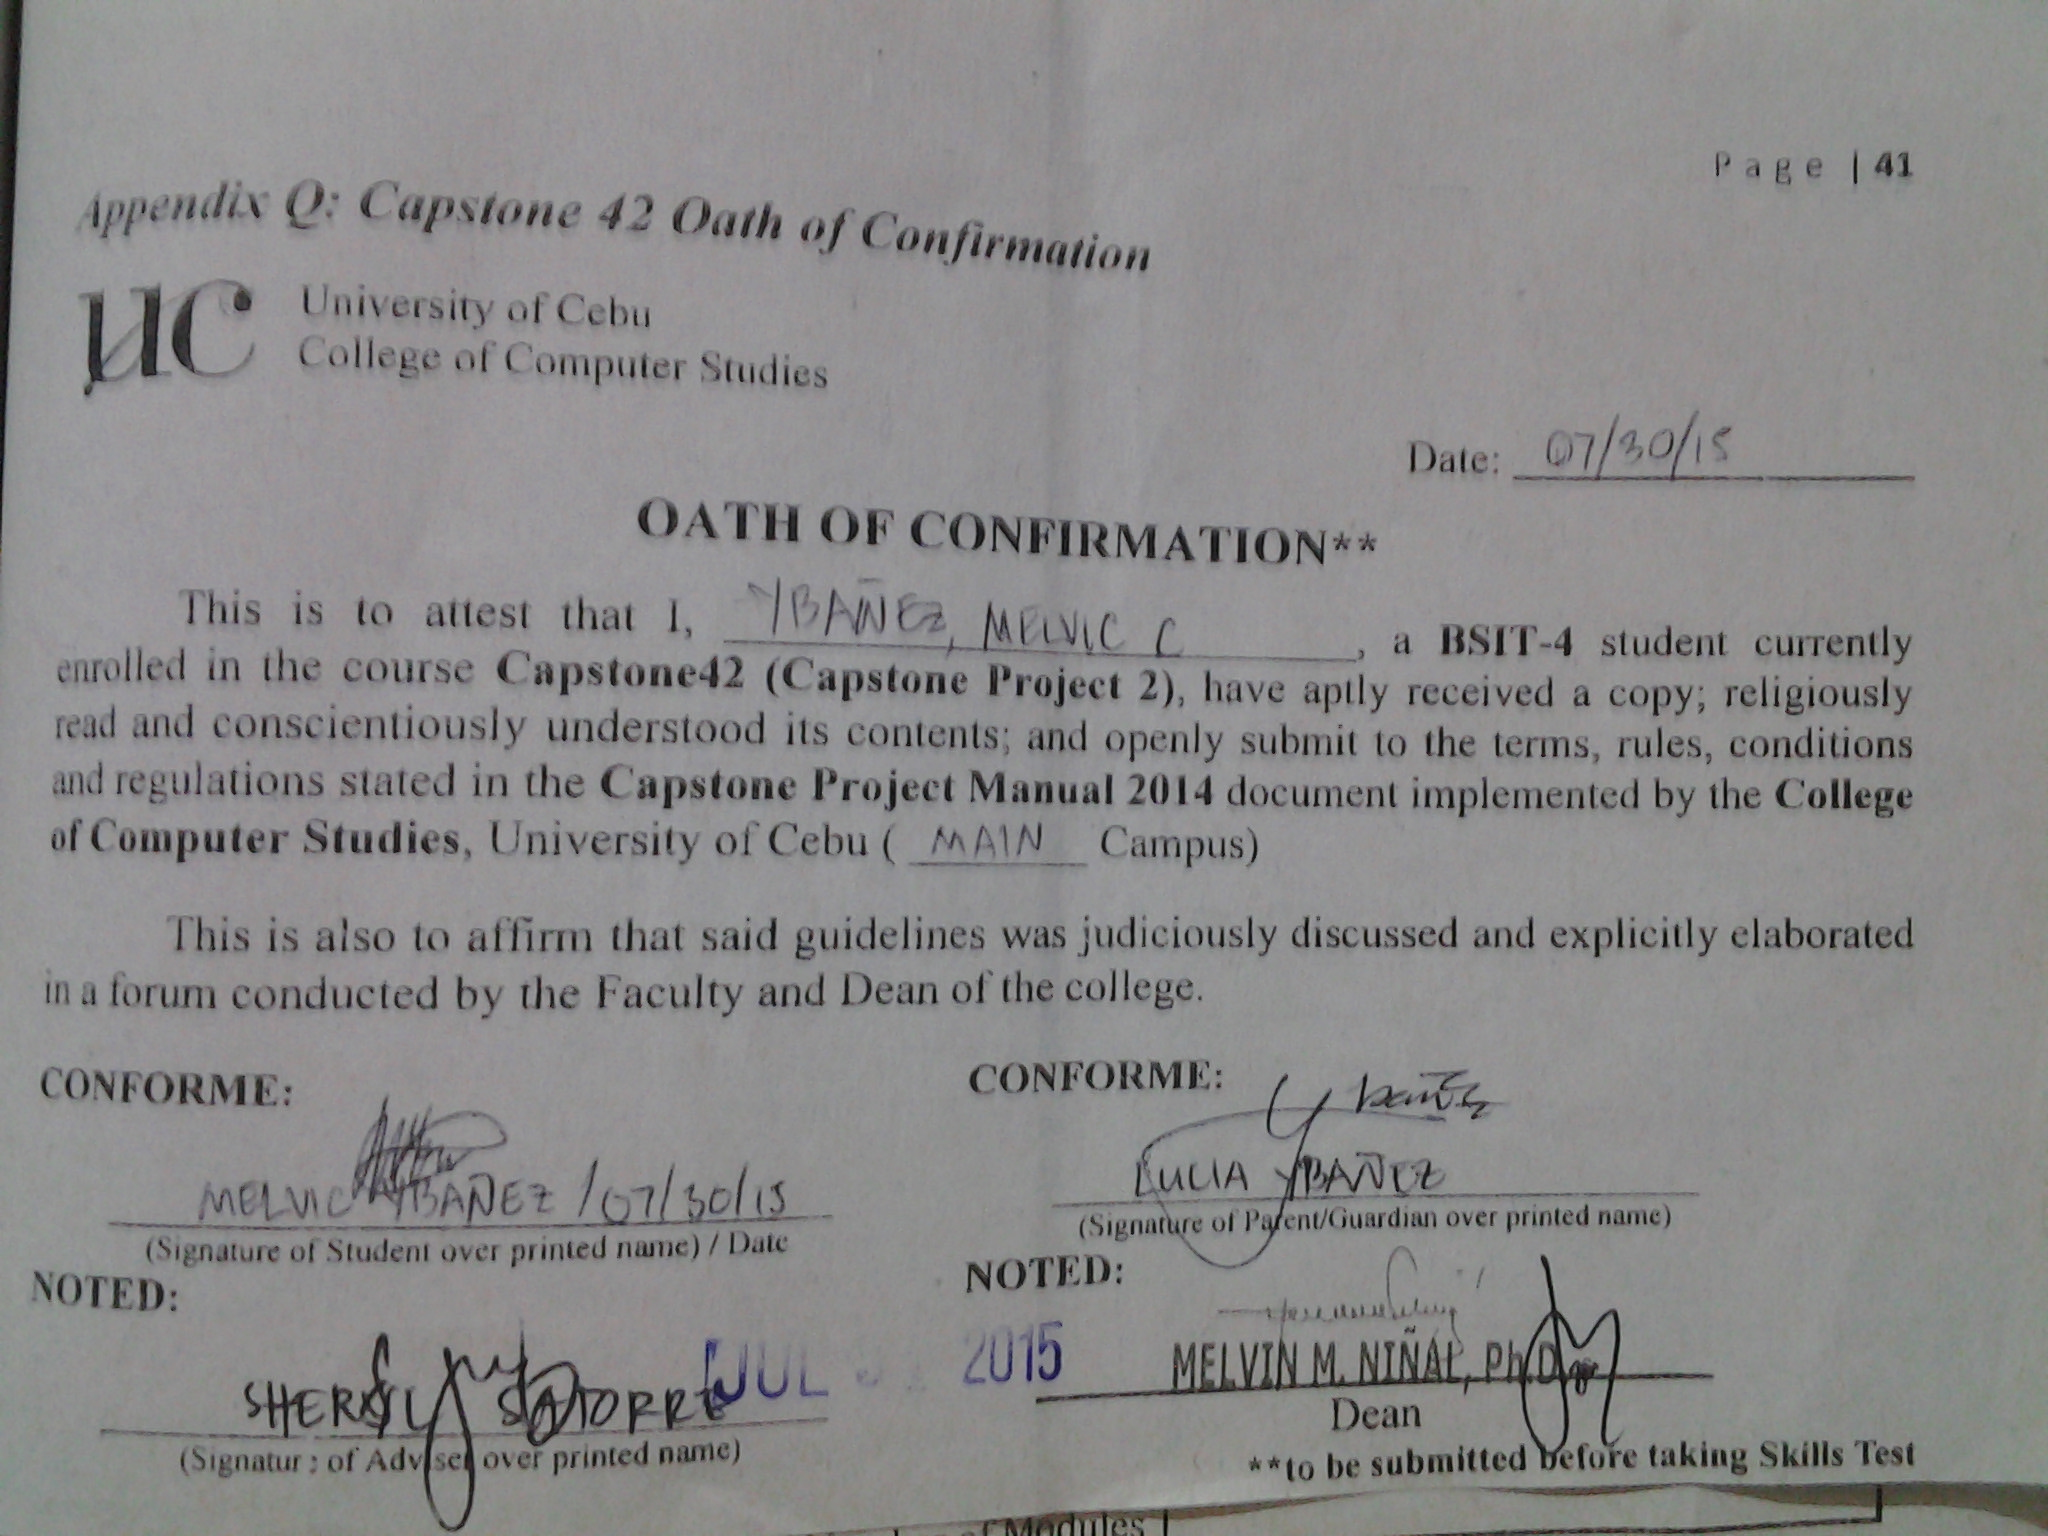
\includegraphics[width=\textwidth]{oath-of-confirmation}
\centering
\end{figure}

\chapter{Oral Defense Hearing Notice}
\begin{figure}[H]
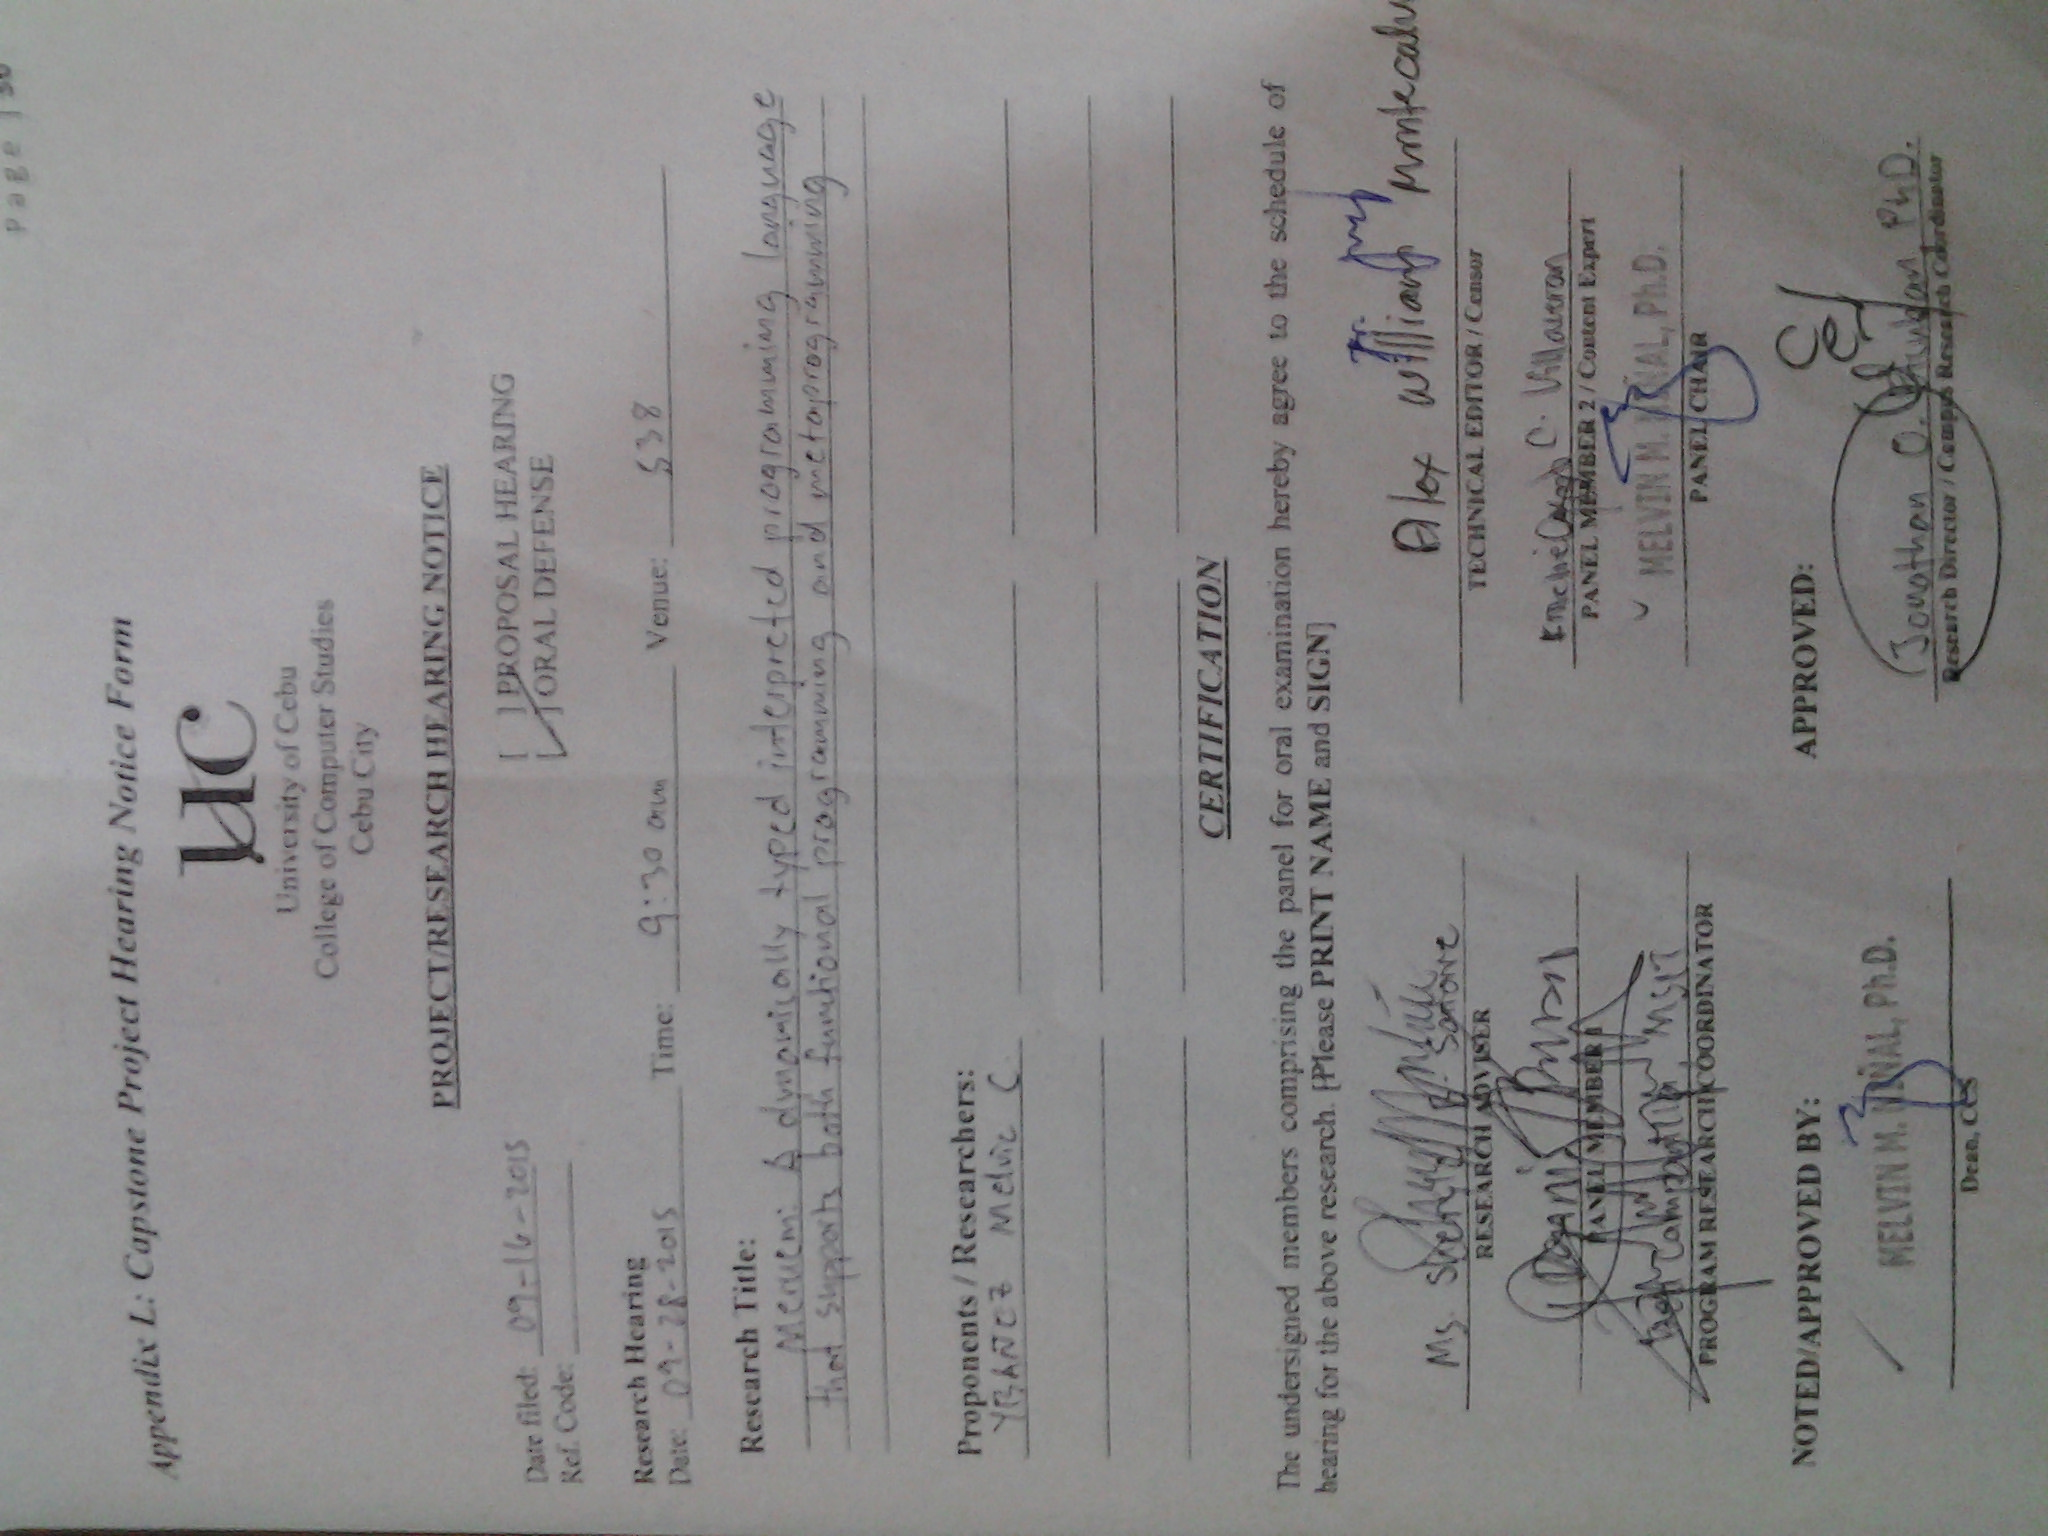
\includegraphics[width=\textwidth, angle=-90]{oral-defense-hearing-notice}
\centering
\end{figure}
	
\end{document}